% VDE Template for EUSAR Papers
% Provided by Barbara Lang und Siegmar Lampe
% University of Bremen, January 2002
% English version by Jens Fischer
% German Aerospace Center (DLR), December 2005
% Additional modifications by Matthias Wei{\ss}
% FGAN, January 2009

%-----------------------------------------------------------------------------
% Type of publication
\documentclass[a4paper,10pt]{article}
%-----------------------------------------------------------------------------
% Other packets: Most packets may be downloaded from www.dante.de and
% "tcilatex.tex" can be found at (December 2005):
% http://www.mackichan.com/techtalk/v30/UsingFloat.htm
% Not all packets are necessarily needed:
\usepackage[T1]{fontenc}
\usepackage[latin1]{inputenc}
%\usepackage{ngerman} % in german language if required
\usepackage[nooneline,bf]{caption} % Figure descriptions from left margin
\usepackage{times}
\usepackage{multicol}
\usepackage{amsmath}
\usepackage{amssymb}
\usepackage{graphicx}
\usepackage{epsfig}
\usepackage{listings}
\usepackage{color}
\usepackage{nameref}
\usepackage{url}
\usepackage{inconsolata}
%\usepackage{paralist}

% Macros for Scientific Word 3.0 documents saved with the LaTeX filter.
%Copyright (C) 1994-97 TCI Software Research, Inc.
\typeout{TCILATEX Macros for Scientific Word 3.0 <05 August 1998>.}
\typeout{NOTICE:  This macro file is NOT proprietary and may be 
freely copied and distributed.}
%
\makeatletter
%
%%%%%%%%%%%%%%%%%%%%%%
% macros for time
\newcount\@hour\newcount\@minute\chardef\@x10\chardef\@xv60
\def\tcitime{
\def\@time{%
  \@minute\time\@hour\@minute\divide\@hour\@xv
  \ifnum\@hour<\@x 0\fi\the\@hour:%
  \multiply\@hour\@xv\advance\@minute-\@hour
  \ifnum\@minute<\@x 0\fi\the\@minute
  }}%

%%%%%%%%%%%%%%%%%%%%%%
% macro for hyperref
\@ifundefined{hyperref}{\def\hyperref#1#2#3#4{#2\ref{#4}#3}}{}

% macro for external program call
\@ifundefined{qExtProgCall}{\def\qExtProgCall#1#2#3#4#5#6{\relax}}{}
%%%%%%%%%%%%%%%%%%%%%%
%
% macros for graphics
%
\def\FILENAME#1{#1}%
%
\def\QCTOpt[#1]#2{%
  \def\QCTOptB{#1}
  \def\QCTOptA{#2}
}
\def\QCTNOpt#1{%
  \def\QCTOptA{#1}
  \let\QCTOptB\empty
}
\def\Qct{%
  \@ifnextchar[{%
    \QCTOpt}{\QCTNOpt}
}
\def\QCBOpt[#1]#2{%
  \def\QCBOptB{#1}
  \def\QCBOptA{#2}
}
\def\QCBNOpt#1{%
  \def\QCBOptA{#1}
  \let\QCBOptB\empty
}
\def\Qcb{%
  \@ifnextchar[{%
    \QCBOpt}{\QCBNOpt}
}
\def\PrepCapArgs{%
  \ifx\QCBOptA\empty
    \ifx\QCTOptA\empty
      {}%
    \else
      \ifx\QCTOptB\empty
        {\QCTOptA}%
      \else
        [\QCTOptB]{\QCTOptA}%
      \fi
    \fi
  \else
    \ifx\QCBOptA\empty
      {}%
    \else
      \ifx\QCBOptB\empty
        {\QCBOptA}%
      \else
        [\QCBOptB]{\QCBOptA}%
      \fi
    \fi
  \fi
}
\newcount\GRAPHICSTYPE
%\GRAPHICSTYPE 0 is for TurboTeX
%\GRAPHICSTYPE 1 is for DVIWindo (PostScript)
%%%(removed)%\GRAPHICSTYPE 2 is for psfig (PostScript)
\GRAPHICSTYPE=\z@
\def\GRAPHICSPS#1{%
 \ifcase\GRAPHICSTYPE%\GRAPHICSTYPE=0
   \special{ps: #1}%
 \or%\GRAPHICSTYPE=1
   \special{language "PS", include "#1"}%
%%%\or%\GRAPHICSTYPE=2
%%%  #1%
 \fi
}%
%
\def\GRAPHICSHP#1{\special{include #1}}%
%
% \graffile{ body }                                  %#1
%          { contentswidth (scalar)  }               %#2
%          { contentsheight (scalar) }               %#3
%          { vertical shift when in-line (scalar) }  %#4
\def\graffile#1#2#3#4{%
%%% \ifnum\GRAPHICSTYPE=\tw@
%%%  %Following if using psfig
%%%  \@ifundefined{psfig}{\input psfig.tex}{}%
%%%  \psfig{file=#1, height=#3, width=#2}%
%%% \else
  %Following for all others
  % JCS - added BOXTHEFRAME, see below
    \bgroup
    \leavevmode
    \@ifundefined{bbl@deactivate}{\def~{\string~}}{\activesoff}
    \raise -#4 \BOXTHEFRAME{%
        \hbox to #2{\raise #3\hbox to #2{\null #1\hfil}}}%
    \egroup
}%
%
% A box for drafts
\def\draftbox#1#2#3#4{%
 \leavevmode\raise -#4 \hbox{%
  \frame{\rlap{\protect\tiny #1}\hbox to #2%
   {\vrule height#3 width\z@ depth\z@\hfil}%
  }%
 }%
}%
%
\newcount\draft
\draft=\z@
\let\nographics=\draft
\newif\ifwasdraft
\wasdraftfalse

%  \GRAPHIC{ body }                                  %#1
%          { draft name }                            %#2
%          { contentswidth (scalar)  }               %#3
%          { contentsheight (scalar) }               %#4
%          { vertical shift when in-line (scalar) }  %#5
\def\GRAPHIC#1#2#3#4#5{%
 \ifnum\draft=\@ne\draftbox{#2}{#3}{#4}{#5}%
  \else\graffile{#1}{#3}{#4}{#5}%
  \fi
 }%
%
\def\addtoLaTeXparams#1{%
    \edef\LaTeXparams{\LaTeXparams #1}}%
%
% JCS -  added a switch BoxFrame that can 
% be set by including X in the frame params.
% If set a box is drawn around the frame.

\newif\ifBoxFrame \BoxFramefalse
\newif\ifOverFrame \OverFramefalse
\newif\ifUnderFrame \UnderFramefalse

\def\BOXTHEFRAME#1{%
   \hbox{%
      \ifBoxFrame
         \frame{#1}%
      \else
         {#1}%
      \fi
   }%
}


\def\doFRAMEparams#1{\BoxFramefalse\OverFramefalse\UnderFramefalse\readFRAMEparams#1\end}%
\def\readFRAMEparams#1{%
 \ifx#1\end%
  \let\next=\relax
  \else
  \ifx#1i\dispkind=\z@\fi
  \ifx#1d\dispkind=\@ne\fi
  \ifx#1f\dispkind=\tw@\fi
  \ifx#1t\addtoLaTeXparams{t}\fi
  \ifx#1b\addtoLaTeXparams{b}\fi
  \ifx#1p\addtoLaTeXparams{p}\fi
  \ifx#1h\addtoLaTeXparams{h}\fi
  \ifx#1X\BoxFrametrue\fi
  \ifx#1O\OverFrametrue\fi
  \ifx#1U\UnderFrametrue\fi
  \ifx#1w
    \ifnum\draft=1\wasdrafttrue\else\wasdraftfalse\fi
    \draft=\@ne
  \fi
  \let\next=\readFRAMEparams
  \fi
 \next
 }%
%
%Macro for In-line graphics object
%   \IFRAME{ contentswidth (scalar)  }               %#1
%          { contentsheight (scalar) }               %#2
%          { vertical shift when in-line (scalar) }  %#3
%          { draft name }                            %#4
%          { body }                                  %#5
%          { caption}                                %#6


\def\IFRAME#1#2#3#4#5#6{%
      \bgroup
      \let\QCTOptA\empty
      \let\QCTOptB\empty
      \let\QCBOptA\empty
      \let\QCBOptB\empty
      #6%
      \parindent=0pt%
      \leftskip=0pt
      \rightskip=0pt
      \setbox0 = \hbox{\QCBOptA}%
      \@tempdima = #1\relax
      \ifOverFrame
          % Do this later
          \typeout{This is not implemented yet}%
          \show\HELP
      \else
         \ifdim\wd0>\@tempdima
            \advance\@tempdima by \@tempdima
            \ifdim\wd0 >\@tempdima
               \textwidth=\@tempdima
               \setbox1 =\vbox{%
                  \noindent\hbox to \@tempdima{\hfill\GRAPHIC{#5}{#4}{#1}{#2}{#3}\hfill}\\%
                  \noindent\hbox to \@tempdima{\parbox[b]{\@tempdima}{\QCBOptA}}%
               }%
               \wd1=\@tempdima
            \else
               \textwidth=\wd0
               \setbox1 =\vbox{%
                 \noindent\hbox to \wd0{\hfill\GRAPHIC{#5}{#4}{#1}{#2}{#3}\hfill}\\%
                 \noindent\hbox{\QCBOptA}%
               }%
               \wd1=\wd0
            \fi
         \else
            %\show\BBB
            \ifdim\wd0>0pt
              \hsize=\@tempdima
              \setbox1 =\vbox{%
                \unskip\GRAPHIC{#5}{#4}{#1}{#2}{0pt}%
                \break
                \unskip\hbox to \@tempdima{\hfill \QCBOptA\hfill}%
              }%
              \wd1=\@tempdima
           \else
              \hsize=\@tempdima
              \setbox1 =\vbox{%
                \unskip\GRAPHIC{#5}{#4}{#1}{#2}{0pt}%
              }%
              \wd1=\@tempdima
           \fi
         \fi
         \@tempdimb=\ht1
         \advance\@tempdimb by \dp1
         \advance\@tempdimb by -#2%
         \advance\@tempdimb by #3%
         \leavevmode
         \raise -\@tempdimb \hbox{\box1}%
      \fi
      \egroup%
}%
%
%Macro for Display graphics object
%   \DFRAME{ contentswidth (scalar)  }               %#1
%          { contentsheight (scalar) }               %#2
%          { draft label }                           %#3
%          { name }                                  %#4
%          { caption}                                %#5
\def\DFRAME#1#2#3#4#5{%
 \begin{center}
     \let\QCTOptA\empty
     \let\QCTOptB\empty
     \let\QCBOptA\empty
     \let\QCBOptB\empty
     \ifOverFrame 
        #5\QCTOptA\par
     \fi
     \GRAPHIC{#4}{#3}{#1}{#2}{\z@}
     \ifUnderFrame 
        \nobreak\par\nobreak#5\QCBOptA
     \fi
 \end{center}%
 }%
%
%Macro for Floating graphic object
%   \FFRAME{ framedata f|i tbph x F|T }              %#1
%          { contentswidth (scalar)  }               %#2
%          { contentsheight (scalar) }               %#3
%          { caption }                               %#4
%          { label }                                 %#5
%          { draft name }                            %#6
%          { body }                                  %#7
\def\FFRAME#1#2#3#4#5#6#7{%
 %If float.sty loaded and float option is 'h', change to 'H'  (gp) 1998/09/05
  \@ifundefined{floatstyle}
    {%floatstyle undefined (and float.sty not present), no change
     \begin{figure}[#1]%
    }
    {%floatstyle DEFINED
	 \ifx#1h%Only the h parameter, change to H
      \begin{figure}[H]%
	 \else
      \begin{figure}[#1]%
	 \fi
	}
  \let\QCTOptA\empty
  \let\QCTOptB\empty
  \let\QCBOptA\empty
  \let\QCBOptB\empty
  \ifOverFrame
    #4
    \ifx\QCTOptA\empty
    \else
      \ifx\QCTOptB\empty
        \caption{\QCTOptA}%
      \else
        \caption[\QCTOptB]{\QCTOptA}%
      \fi
    \fi
    \ifUnderFrame\else
      \label{#5}%
    \fi
  \else
    \UnderFrametrue%
  \fi
  \begin{center}\GRAPHIC{#7}{#6}{#2}{#3}{\z@}\end{center}%
  \ifUnderFrame
    #4
    \ifx\QCBOptA\empty
      \caption{}%
    \else
      \ifx\QCBOptB\empty
        \caption{\QCBOptA}%
      \else
        \caption[\QCBOptB]{\QCBOptA}%
      \fi
    \fi
    \label{#5}%
  \fi
  \end{figure}%
 }%
%
%
%    \FRAME{ framedata f|i tbph x F|T }              %#1
%          { contentswidth (scalar)  }               %#2
%          { contentsheight (scalar) }               %#3
%          { vertical shift when in-line (scalar) }  %#4
%          { caption }                               %#5
%          { label }                                 %#6
%          { name }                                  %#7
%          { body }                                  %#8
%
%    framedata is a string which can contain the following
%    characters: idftbphxFT
%    Their meaning is as follows:
%             i, d or f : in-line, display, or floating
%             t,b,p,h   : LaTeX floating placement options
%             x         : fit contents box to contents
%             F or T    : Figure or Table. 
%                         Later this can expand
%                         to a more general float class.
%
%
\newcount\dispkind%

\def\makeactives{
  \catcode`\"=\active
  \catcode`\;=\active
  \catcode`\:=\active
  \catcode`\'=\active
  \catcode`\~=\active
}
\bgroup
   \makeactives
   \gdef\activesoff{%
      \def"{\string"}
      \def;{\string;}
      \def:{\string:}
      \def'{\string'}
      \def~{\string~}
      %\bbl@deactivate{"}%
      %\bbl@deactivate{;}%
      %\bbl@deactivate{:}%
      %\bbl@deactivate{'}%
    }
\egroup

\def\FRAME#1#2#3#4#5#6#7#8{%
 \bgroup
 \ifnum\draft=\@ne
   \wasdrafttrue
 \else
   \wasdraftfalse%
 \fi
 \def\LaTeXparams{}%
 \dispkind=\z@
 \def\LaTeXparams{}%
 \doFRAMEparams{#1}%
 \ifnum\dispkind=\z@\IFRAME{#2}{#3}{#4}{#7}{#8}{#5}\else
  \ifnum\dispkind=\@ne\DFRAME{#2}{#3}{#7}{#8}{#5}\else
   \ifnum\dispkind=\tw@
    \edef\@tempa{\noexpand\FFRAME{\LaTeXparams}}%
    \@tempa{#2}{#3}{#5}{#6}{#7}{#8}%
    \fi
   \fi
  \fi
  \ifwasdraft\draft=1\else\draft=0\fi{}%
  \egroup
 }%
%
% This macro added to let SW gobble a parameter that
% should not be passed on and expanded. 

\def\TEXUX#1{"texux"}

%
% Macros for text attributes:
%
\def\BF#1{{\bf {#1}}}%
\def\NEG#1{\leavevmode\hbox{\rlap{\thinspace/}{$#1$}}}%
%
%%%%%%%%%%%%%%%%%%%%%%%%%%%%%%%%%%%%%%%%%%%%%%%%%%%%%%%%%%%%%%%%%%%%%%%%
%
%
% macros for user - defined functions
\def\limfunc#1{\mathop{\rm #1}}%
\def\func#1{\mathop{\rm #1}\nolimits}%
% macro for unit names
\def\unit#1{\mathop{\rm #1}\nolimits}%

%
% miscellaneous 
\long\def\QQQ#1#2{%
     \long\expandafter\def\csname#1\endcsname{#2}}%
\@ifundefined{QTP}{\def\QTP#1{}}{}
\@ifundefined{QEXCLUDE}{\def\QEXCLUDE#1{}}{}
\@ifundefined{Qlb}{\def\Qlb#1{#1}}{}
\@ifundefined{Qlt}{\def\Qlt#1{#1}}{}
\def\QWE{}%
\long\def\QQA#1#2{}%
\def\QTR#1#2{{\csname#1\endcsname #2}}%(gp) Is this the best?
\long\def\TeXButton#1#2{#2}%
\long\def\QSubDoc#1#2{#2}%
\def\EXPAND#1[#2]#3{}%
\def\NOEXPAND#1[#2]#3{}%
\def\PROTECTED{}%
\def\LaTeXparent#1{}%
\def\ChildStyles#1{}%
\def\ChildDefaults#1{}%
\def\QTagDef#1#2#3{}%

% Constructs added with Scientific Notebook
\@ifundefined{correctchoice}{\def\correctchoice{\relax}}{}
\@ifundefined{HTML}{\def\HTML#1{\relax}}{}
\@ifundefined{TCIIcon}{\def\TCIIcon#1#2#3#4{\relax}}{}
\if@compatibility
  \typeout{Not defining UNICODE or CustomNote commands for LaTeX 2.09.}
\else
  \providecommand{\UNICODE}[2][]{}
  \providecommand{\CustomNote}[3][]{\marginpar{#3}}
\fi

%
% Macros for style editor docs
\@ifundefined{StyleEditBeginDoc}{\def\StyleEditBeginDoc{\relax}}{}
%
% Macros for footnotes
\def\QQfnmark#1{\footnotemark}
\def\QQfntext#1#2{\addtocounter{footnote}{#1}\footnotetext{#2}}
%
% Macros for indexing.
%
\@ifundefined{TCIMAKEINDEX}{}{\makeindex}%
%
% Attempts to avoid problems with other styles
\@ifundefined{abstract}{%
 \def\abstract{%
  \if@twocolumn
   \section*{Abstract (Not appropriate in this style!)}%
   \else \small 
   \begin{center}{\bf Abstract\vspace{-.5em}\vspace{\z@}}\end{center}%
   \quotation 
   \fi
  }%
 }{%
 }%
\@ifundefined{endabstract}{\def\endabstract
  {\if@twocolumn\else\endquotation\fi}}{}%
\@ifundefined{maketitle}{\def\maketitle#1{}}{}%
\@ifundefined{affiliation}{\def\affiliation#1{}}{}%
\@ifundefined{proof}{\def\proof{\noindent{\bfseries Proof. }}}{}%
\@ifundefined{endproof}{\def\endproof{\mbox{\ \rule{.1in}{.1in}}}}{}%
\@ifundefined{newfield}{\def\newfield#1#2{}}{}%
\@ifundefined{chapter}{\def\chapter#1{\par(Chapter head:)#1\par }%
 \newcount\c@chapter}{}%
\@ifundefined{part}{\def\part#1{\par(Part head:)#1\par }}{}%
\@ifundefined{section}{\def\section#1{\par(Section head:)#1\par }}{}%
\@ifundefined{subsection}{\def\subsection#1%
 {\par(Subsection head:)#1\par }}{}%
\@ifundefined{subsubsection}{\def\subsubsection#1%
 {\par(Subsubsection head:)#1\par }}{}%
\@ifundefined{paragraph}{\def\paragraph#1%
 {\par(Subsubsubsection head:)#1\par }}{}%
\@ifundefined{subparagraph}{\def\subparagraph#1%
 {\par(Subsubsubsubsection head:)#1\par }}{}%
%%%%%%%%%%%%%%%%%%%%%%%%%%%%%%%%%%%%%%%%%%%%%%%%%%%%%%%%%%%%%%%%%%%%%%%%
% These symbols are not recognized by LaTeX
\@ifundefined{therefore}{\def\therefore{}}{}%
\@ifundefined{backepsilon}{\def\backepsilon{}}{}%
\@ifundefined{yen}{\def\yen{\hbox{\rm\rlap=Y}}}{}%
\@ifundefined{registered}{%
   \def\registered{\relax\ifmmode{}\r@gistered
                    \else$\m@th\r@gistered$\fi}%
 \def\r@gistered{^{\ooalign
  {\hfil\raise.07ex\hbox{$\scriptstyle\rm\text{R}$}\hfil\crcr
  \mathhexbox20D}}}}{}%
\@ifundefined{Eth}{\def\Eth{}}{}%
\@ifundefined{eth}{\def\eth{}}{}%
\@ifundefined{Thorn}{\def\Thorn{}}{}%
\@ifundefined{thorn}{\def\thorn{}}{}%
% A macro to allow any symbol that requires math to appear in text
\def\TEXTsymbol#1{\mbox{$#1$}}%
\@ifundefined{degree}{\def\degree{{}^{\circ}}}{}%
%
% macros for T3TeX files
\newdimen\theight
\def\Column{%
 \vadjust{\setbox\z@=\hbox{\scriptsize\quad\quad tcol}%
  \theight=\ht\z@\advance\theight by \dp\z@\advance\theight by \lineskip
  \kern -\theight \vbox to \theight{%
   \rightline{\rlap{\box\z@}}%
   \vss
   }%
  }%
 }%
%
\def\qed{%
 \ifhmode\unskip\nobreak\fi\ifmmode\ifinner\else\hskip5\p@\fi\fi
 \hbox{\hskip5\p@\vrule width4\p@ height6\p@ depth1.5\p@\hskip\p@}%
 }%
%
\def\cents{\hbox{\rm\rlap/c}}%
\def\miss{\hbox{\vrule height2\p@ width 2\p@ depth\z@}}%
%
\def\vvert{\Vert}%           %always translated to \left| or \right|
%
\def\tcol#1{{\baselineskip=6\p@ \vcenter{#1}} \Column}  %
%
\def\dB{\hbox{{}}}%                 %dummy entry in column 
\def\mB#1{\hbox{$#1$}}%             %column entry
\def\nB#1{\hbox{#1}}%               %column entry (not math)
%
\@ifundefined{note}{\def\note{$^{\dag}}}{}%
%

\def\newfmtname{LaTeX2e}
% No longer load latexsym.  This is now handled by SWP, which uses amsfonts if necessary

\ifx\fmtname\newfmtname
  \DeclareOldFontCommand{\rm}{\normalfont\rmfamily}{\mathrm}
  \DeclareOldFontCommand{\sf}{\normalfont\sffamily}{\mathsf}
  \DeclareOldFontCommand{\tt}{\normalfont\ttfamily}{\mathtt}
  \DeclareOldFontCommand{\bf}{\normalfont\bfseries}{\mathbf}
  \DeclareOldFontCommand{\it}{\normalfont\itshape}{\mathit}
  \DeclareOldFontCommand{\sl}{\normalfont\slshape}{\@nomath\sl}
  \DeclareOldFontCommand{\sc}{\normalfont\scshape}{\@nomath\sc}
\fi

%
% Greek bold macros
% Redefine all of the math symbols 
% which might be bolded	 - there are 
% probably others to add to this list

\def\alpha{{\Greekmath 010B}}%
\def\beta{{\Greekmath 010C}}%
\def\gamma{{\Greekmath 010D}}%
\def\delta{{\Greekmath 010E}}%
\def\epsilon{{\Greekmath 010F}}%
\def\zeta{{\Greekmath 0110}}%
\def\eta{{\Greekmath 0111}}%
\def\theta{{\Greekmath 0112}}%
\def\iota{{\Greekmath 0113}}%
\def\kappa{{\Greekmath 0114}}%
\def\lambda{{\Greekmath 0115}}%
\def\mu{{\Greekmath 0116}}%
\def\nu{{\Greekmath 0117}}%
\def\xi{{\Greekmath 0118}}%
\def\pi{{\Greekmath 0119}}%
\def\rho{{\Greekmath 011A}}%
\def\sigma{{\Greekmath 011B}}%
\def\tau{{\Greekmath 011C}}%
\def\upsilon{{\Greekmath 011D}}%
\def\phi{{\Greekmath 011E}}%
\def\chi{{\Greekmath 011F}}%
\def\psi{{\Greekmath 0120}}%
\def\omega{{\Greekmath 0121}}%
\def\varepsilon{{\Greekmath 0122}}%
\def\vartheta{{\Greekmath 0123}}%
\def\varpi{{\Greekmath 0124}}%
\def\varrho{{\Greekmath 0125}}%
\def\varsigma{{\Greekmath 0126}}%
\def\varphi{{\Greekmath 0127}}%

\def\nabla{{\Greekmath 0272}}
\def\FindBoldGroup{%
   {\setbox0=\hbox{$\mathbf{x\global\edef\theboldgroup{\the\mathgroup}}$}}%
}

\def\Greekmath#1#2#3#4{%
    \if@compatibility
        \ifnum\mathgroup=\symbold
           \mathchoice{\mbox{\boldmath$\displaystyle\mathchar"#1#2#3#4$}}%
                      {\mbox{\boldmath$\textstyle\mathchar"#1#2#3#4$}}%
                      {\mbox{\boldmath$\scriptstyle\mathchar"#1#2#3#4$}}%
                      {\mbox{\boldmath$\scriptscriptstyle\mathchar"#1#2#3#4$}}%
        \else
           \mathchar"#1#2#3#4% 
        \fi 
    \else 
        \FindBoldGroup
        \ifnum\mathgroup=\theboldgroup % For 2e
           \mathchoice{\mbox{\boldmath$\displaystyle\mathchar"#1#2#3#4$}}%
                      {\mbox{\boldmath$\textstyle\mathchar"#1#2#3#4$}}%
                      {\mbox{\boldmath$\scriptstyle\mathchar"#1#2#3#4$}}%
                      {\mbox{\boldmath$\scriptscriptstyle\mathchar"#1#2#3#4$}}%
        \else
           \mathchar"#1#2#3#4% 
        \fi     	    
	  \fi}

\newif\ifGreekBold  \GreekBoldfalse
\let\SAVEPBF=\pbf
\def\pbf{\GreekBoldtrue\SAVEPBF}%
%

\@ifundefined{theorem}{\newtheorem{theorem}{Theorem}}{}
\@ifundefined{lemma}{\newtheorem{lemma}[theorem]{Lemma}}{}
\@ifundefined{corollary}{\newtheorem{corollary}[theorem]{Corollary}}{}
\@ifundefined{conjecture}{\newtheorem{conjecture}[theorem]{Conjecture}}{}
\@ifundefined{proposition}{\newtheorem{proposition}[theorem]{Proposition}}{}
\@ifundefined{axiom}{\newtheorem{axiom}{Axiom}}{}
\@ifundefined{remark}{\newtheorem{remark}{Remark}}{}
\@ifundefined{example}{\newtheorem{example}{Example}}{}
\@ifundefined{exercise}{\newtheorem{exercise}{Exercise}}{}
\@ifundefined{definition}{\newtheorem{definition}{Definition}}{}


\@ifundefined{mathletters}{%
  %\def\theequation{\arabic{equation}}
  \newcounter{equationnumber}  
  \def\mathletters{%
     \addtocounter{equation}{1}
     \edef\@currentlabel{\theequation}%
     \setcounter{equationnumber}{\c@equation}
     \setcounter{equation}{0}%
     \edef\theequation{\@currentlabel\noexpand\alph{equation}}%
  }
  \def\endmathletters{%
     \setcounter{equation}{\value{equationnumber}}%
  }
}{}

%Logos
\@ifundefined{BibTeX}{%
    \def\BibTeX{{\rm B\kern-.05em{\sc i\kern-.025em b}\kern-.08em
                 T\kern-.1667em\lower.7ex\hbox{E}\kern-.125emX}}}{}%
\@ifundefined{AmS}%
    {\def\AmS{{\protect\usefont{OMS}{cmsy}{m}{n}%
                A\kern-.1667em\lower.5ex\hbox{M}\kern-.125emS}}}{}%
\@ifundefined{AmSTeX}{\def\AmSTeX{\protect\AmS-\protect\TeX\@}}{}%
%

% This macro is a fix to eqnarray
\def\@@eqncr{\let\@tempa\relax
    \ifcase\@eqcnt \def\@tempa{& & &}\or \def\@tempa{& &}%
      \else \def\@tempa{&}\fi
     \@tempa
     \if@eqnsw
        \iftag@
           \@taggnum
        \else
           \@eqnnum\stepcounter{equation}%
        \fi
     \fi
     \global\tag@false
     \global\@eqnswtrue
     \global\@eqcnt\z@\cr}


\def\TCItag{\@ifnextchar*{\@TCItagstar}{\@TCItag}}
\def\@TCItag#1{%
    \global\tag@true
    \global\def\@taggnum{(#1)}}
\def\@TCItagstar*#1{%
    \global\tag@true
    \global\def\@taggnum{#1}}
%
%%%%%%%%%%%%%%%%%%%%%%%%%%%%%%%%%%%%%%%%%%%%%%%%%%%%%%%%%%%%%%%%%%%%%
%
\def\tfrac#1#2{{\textstyle {#1 \over #2}}}%
\def\dfrac#1#2{{\displaystyle {#1 \over #2}}}%
\def\binom#1#2{{#1 \choose #2}}%
\def\tbinom#1#2{{\textstyle {#1 \choose #2}}}%
\def\dbinom#1#2{{\displaystyle {#1 \choose #2}}}%
\def\QATOP#1#2{{#1 \atop #2}}%
\def\QTATOP#1#2{{\textstyle {#1 \atop #2}}}%
\def\QDATOP#1#2{{\displaystyle {#1 \atop #2}}}%
\def\QABOVE#1#2#3{{#2 \above#1 #3}}%
\def\QTABOVE#1#2#3{{\textstyle {#2 \above#1 #3}}}%
\def\QDABOVE#1#2#3{{\displaystyle {#2 \above#1 #3}}}%
\def\QOVERD#1#2#3#4{{#3 \overwithdelims#1#2 #4}}%
\def\QTOVERD#1#2#3#4{{\textstyle {#3 \overwithdelims#1#2 #4}}}%
\def\QDOVERD#1#2#3#4{{\displaystyle {#3 \overwithdelims#1#2 #4}}}%
\def\QATOPD#1#2#3#4{{#3 \atopwithdelims#1#2 #4}}%
\def\QTATOPD#1#2#3#4{{\textstyle {#3 \atopwithdelims#1#2 #4}}}%
\def\QDATOPD#1#2#3#4{{\displaystyle {#3 \atopwithdelims#1#2 #4}}}%
\def\QABOVED#1#2#3#4#5{{#4 \abovewithdelims#1#2#3 #5}}%
\def\QTABOVED#1#2#3#4#5{{\textstyle 
   {#4 \abovewithdelims#1#2#3 #5}}}%
\def\QDABOVED#1#2#3#4#5{{\displaystyle 
   {#4 \abovewithdelims#1#2#3 #5}}}%
%
% Macros for text size operators:
%
\def\tint{\mathop{\textstyle \int}}%
\def\tiint{\mathop{\textstyle \iint }}%
\def\tiiint{\mathop{\textstyle \iiint }}%
\def\tiiiint{\mathop{\textstyle \iiiint }}%
\def\tidotsint{\mathop{\textstyle \idotsint }}%
\def\toint{\mathop{\textstyle \oint}}%
\def\tsum{\mathop{\textstyle \sum }}%
\def\tprod{\mathop{\textstyle \prod }}%
\def\tbigcap{\mathop{\textstyle \bigcap }}%
\def\tbigwedge{\mathop{\textstyle \bigwedge }}%
\def\tbigoplus{\mathop{\textstyle \bigoplus }}%
\def\tbigodot{\mathop{\textstyle \bigodot }}%
\def\tbigsqcup{\mathop{\textstyle \bigsqcup }}%
\def\tcoprod{\mathop{\textstyle \coprod }}%
\def\tbigcup{\mathop{\textstyle \bigcup }}%
\def\tbigvee{\mathop{\textstyle \bigvee }}%
\def\tbigotimes{\mathop{\textstyle \bigotimes }}%
\def\tbiguplus{\mathop{\textstyle \biguplus }}%
%
%
%Macros for display size operators:
%
\def\dint{\mathop{\displaystyle \int}}%
\def\diint{\mathop{\displaystyle \iint }}%
\def\diiint{\mathop{\displaystyle \iiint }}%
\def\diiiint{\mathop{\displaystyle \iiiint }}%
\def\didotsint{\mathop{\displaystyle \idotsint }}%
\def\doint{\mathop{\displaystyle \oint}}%
\def\dsum{\mathop{\displaystyle \sum }}%
\def\dprod{\mathop{\displaystyle \prod }}%
\def\dbigcap{\mathop{\displaystyle \bigcap }}%
\def\dbigwedge{\mathop{\displaystyle \bigwedge }}%
\def\dbigoplus{\mathop{\displaystyle \bigoplus }}%
\def\dbigodot{\mathop{\displaystyle \bigodot }}%
\def\dbigsqcup{\mathop{\displaystyle \bigsqcup }}%
\def\dcoprod{\mathop{\displaystyle \coprod }}%
\def\dbigcup{\mathop{\displaystyle \bigcup }}%
\def\dbigvee{\mathop{\displaystyle \bigvee }}%
\def\dbigotimes{\mathop{\displaystyle \bigotimes }}%
\def\dbiguplus{\mathop{\displaystyle \biguplus }}%

%%%%%%%%%%%%%%%%%%%%%%%%%%%%%%%%%%%%%%%%%%%%%%%%%%%%%%%%%%%%%%%%%%%%%%%
% NOTE: The rest of this file is read only if amstex has not been
% loaded.  This section is used to define amstex constructs in the
% event they have not been defined.
%
%
\ifx\ds@amstex\relax
   \message{amstex already loaded}\makeatother\endinput% 2.09 compatability
\else
   \@ifpackageloaded{amsmath}%
      {\message{amsmath already loaded}\makeatother\endinput}
      {}
   \@ifpackageloaded{amstex}%
      {\message{amstex already loaded}\makeatother\endinput}
      {}
   \@ifpackageloaded{amsgen}%
      {\message{amsgen already loaded}\makeatother\endinput}
      {}
\fi
%%%%%%%%%%%%%%%%%%%%%%%%%%%%%%%%%%%%%%%%%%%%%%%%%%%%%%%%%%%%%%%%%%%%%%%%
%%
%
%
%  Macros to define some AMS LaTeX constructs when 
%  AMS LaTeX has not been loaded
% 
% These macros are copied from the AMS-TeX package for doing
% multiple integrals.
%
\let\DOTSI\relax
\def\RIfM@{\relax\ifmmode}%
\def\FN@{\futurelet\next}%
\newcount\intno@
\def\iint{\DOTSI\intno@\tw@\FN@\ints@}%
\def\iiint{\DOTSI\intno@\thr@@\FN@\ints@}%
\def\iiiint{\DOTSI\intno@4 \FN@\ints@}%
\def\idotsint{\DOTSI\intno@\z@\FN@\ints@}%
\def\ints@{\findlimits@\ints@@}%
\newif\iflimtoken@
\newif\iflimits@
\def\findlimits@{\limtoken@true\ifx\next\limits\limits@true
 \else\ifx\next\nolimits\limits@false\else
 \limtoken@false\ifx\ilimits@\nolimits\limits@false\else
 \ifinner\limits@false\else\limits@true\fi\fi\fi\fi}%
\def\multint@{\int\ifnum\intno@=\z@\intdots@                          %1
 \else\intkern@\fi                                                    %2
 \ifnum\intno@>\tw@\int\intkern@\fi                                   %3
 \ifnum\intno@>\thr@@\int\intkern@\fi                                 %4
 \int}%                                                               %5
\def\multintlimits@{\intop\ifnum\intno@=\z@\intdots@\else\intkern@\fi
 \ifnum\intno@>\tw@\intop\intkern@\fi
 \ifnum\intno@>\thr@@\intop\intkern@\fi\intop}%
\def\intic@{%
    \mathchoice{\hskip.5em}{\hskip.4em}{\hskip.4em}{\hskip.4em}}%
\def\negintic@{\mathchoice
 {\hskip-.5em}{\hskip-.4em}{\hskip-.4em}{\hskip-.4em}}%
\def\ints@@{\iflimtoken@                                              %1
 \def\ints@@@{\iflimits@\negintic@
   \mathop{\intic@\multintlimits@}\limits                             %2
  \else\multint@\nolimits\fi                                          %3
  \eat@}%                                                             %4
 \else                                                                %5
 \def\ints@@@{\iflimits@\negintic@
  \mathop{\intic@\multintlimits@}\limits\else
  \multint@\nolimits\fi}\fi\ints@@@}%
\def\intkern@{\mathchoice{\!\!\!}{\!\!}{\!\!}{\!\!}}%
\def\plaincdots@{\mathinner{\cdotp\cdotp\cdotp}}%
\def\intdots@{\mathchoice{\plaincdots@}%
 {{\cdotp}\mkern1.5mu{\cdotp}\mkern1.5mu{\cdotp}}%
 {{\cdotp}\mkern1mu{\cdotp}\mkern1mu{\cdotp}}%
 {{\cdotp}\mkern1mu{\cdotp}\mkern1mu{\cdotp}}}%
%
%
%  These macros are for doing the AMS \text{} construct
%
\def\RIfM@{\relax\protect\ifmmode}
\def\text{\RIfM@\expandafter\text@\else\expandafter\mbox\fi}
\let\nfss@text\text
\def\text@#1{\mathchoice
   {\textdef@\displaystyle\f@size{#1}}%
   {\textdef@\textstyle\tf@size{\firstchoice@false #1}}%
   {\textdef@\textstyle\sf@size{\firstchoice@false #1}}%
   {\textdef@\textstyle \ssf@size{\firstchoice@false #1}}%
   \glb@settings}

\def\textdef@#1#2#3{\hbox{{%
                    \everymath{#1}%
                    \let\f@size#2\selectfont
                    #3}}}
\newif\iffirstchoice@
\firstchoice@true
%
%These are the AMS constructs for multiline limits.
%
\def\Let@{\relax\iffalse{\fi\let\\=\cr\iffalse}\fi}%
\def\vspace@{\def\vspace##1{\crcr\noalign{\vskip##1\relax}}}%
\def\multilimits@{\bgroup\vspace@\Let@
 \baselineskip\fontdimen10 \scriptfont\tw@
 \advance\baselineskip\fontdimen12 \scriptfont\tw@
 \lineskip\thr@@\fontdimen8 \scriptfont\thr@@
 \lineskiplimit\lineskip
 \vbox\bgroup\ialign\bgroup\hfil$\m@th\scriptstyle{##}$\hfil\crcr}%
\def\Sb{_\multilimits@}%
\def\endSb{\crcr\egroup\egroup\egroup}%
\def\Sp{^\multilimits@}%
\let\endSp\endSb
%
%
%These are AMS constructs for horizontal arrows
%
\newdimen\ex@
\ex@.2326ex
\def\rightarrowfill@#1{$#1\m@th\mathord-\mkern-6mu\cleaders
 \hbox{$#1\mkern-2mu\mathord-\mkern-2mu$}\hfill
 \mkern-6mu\mathord\rightarrow$}%
\def\leftarrowfill@#1{$#1\m@th\mathord\leftarrow\mkern-6mu\cleaders
 \hbox{$#1\mkern-2mu\mathord-\mkern-2mu$}\hfill\mkern-6mu\mathord-$}%
\def\leftrightarrowfill@#1{$#1\m@th\mathord\leftarrow
\mkern-6mu\cleaders
 \hbox{$#1\mkern-2mu\mathord-\mkern-2mu$}\hfill
 \mkern-6mu\mathord\rightarrow$}%
\def\overrightarrow{\mathpalette\overrightarrow@}%
\def\overrightarrow@#1#2{\vbox{\ialign{##\crcr\rightarrowfill@#1\crcr
 \noalign{\kern-\ex@\nointerlineskip}$\m@th\hfil#1#2\hfil$\crcr}}}%
\let\overarrow\overrightarrow
\def\overleftarrow{\mathpalette\overleftarrow@}%
\def\overleftarrow@#1#2{\vbox{\ialign{##\crcr\leftarrowfill@#1\crcr
 \noalign{\kern-\ex@\nointerlineskip}$\m@th\hfil#1#2\hfil$\crcr}}}%
\def\overleftrightarrow{\mathpalette\overleftrightarrow@}%
\def\overleftrightarrow@#1#2{\vbox{\ialign{##\crcr
   \leftrightarrowfill@#1\crcr
 \noalign{\kern-\ex@\nointerlineskip}$\m@th\hfil#1#2\hfil$\crcr}}}%
\def\underrightarrow{\mathpalette\underrightarrow@}%
\def\underrightarrow@#1#2{\vtop{\ialign{##\crcr$\m@th\hfil#1#2\hfil
  $\crcr\noalign{\nointerlineskip}\rightarrowfill@#1\crcr}}}%
\let\underarrow\underrightarrow
\def\underleftarrow{\mathpalette\underleftarrow@}%
\def\underleftarrow@#1#2{\vtop{\ialign{##\crcr$\m@th\hfil#1#2\hfil
  $\crcr\noalign{\nointerlineskip}\leftarrowfill@#1\crcr}}}%
\def\underleftrightarrow{\mathpalette\underleftrightarrow@}%
\def\underleftrightarrow@#1#2{\vtop{\ialign{##\crcr$\m@th
  \hfil#1#2\hfil$\crcr
 \noalign{\nointerlineskip}\leftrightarrowfill@#1\crcr}}}%
%%%%%%%%%%%%%%%%%%%%%

\def\qopnamewl@#1{\mathop{\operator@font#1}\nlimits@}
\let\nlimits@\displaylimits
\def\setboxz@h{\setbox\z@\hbox}


\def\varlim@#1#2{\mathop{\vtop{\ialign{##\crcr
 \hfil$#1\m@th\operator@font lim$\hfil\crcr
 \noalign{\nointerlineskip}#2#1\crcr
 \noalign{\nointerlineskip\kern-\ex@}\crcr}}}}

 \def\rightarrowfill@#1{\m@th\setboxz@h{$#1-$}\ht\z@\z@
  $#1\copy\z@\mkern-6mu\cleaders
  \hbox{$#1\mkern-2mu\box\z@\mkern-2mu$}\hfill
  \mkern-6mu\mathord\rightarrow$}
\def\leftarrowfill@#1{\m@th\setboxz@h{$#1-$}\ht\z@\z@
  $#1\mathord\leftarrow\mkern-6mu\cleaders
  \hbox{$#1\mkern-2mu\copy\z@\mkern-2mu$}\hfill
  \mkern-6mu\box\z@$}


\def\projlim{\qopnamewl@{proj\,lim}}
\def\injlim{\qopnamewl@{inj\,lim}}
\def\varinjlim{\mathpalette\varlim@\rightarrowfill@}
\def\varprojlim{\mathpalette\varlim@\leftarrowfill@}
\def\varliminf{\mathpalette\varliminf@{}}
\def\varliminf@#1{\mathop{\underline{\vrule\@depth.2\ex@\@width\z@
   \hbox{$#1\m@th\operator@font lim$}}}}
\def\varlimsup{\mathpalette\varlimsup@{}}
\def\varlimsup@#1{\mathop{\overline
  {\hbox{$#1\m@th\operator@font lim$}}}}

%
%Companion to stackrel
\def\stackunder#1#2{\mathrel{\mathop{#2}\limits_{#1}}}%
%
%
% These are AMS environments that will be defined to
% be verbatims if amstex has not actually been 
% loaded
%
%
\begingroup \catcode `|=0 \catcode `[= 1
\catcode`]=2 \catcode `\{=12 \catcode `\}=12
\catcode`\\=12 
|gdef|@alignverbatim#1\end{align}[#1|end[align]]
|gdef|@salignverbatim#1\end{align*}[#1|end[align*]]

|gdef|@alignatverbatim#1\end{alignat}[#1|end[alignat]]
|gdef|@salignatverbatim#1\end{alignat*}[#1|end[alignat*]]

|gdef|@xalignatverbatim#1\end{xalignat}[#1|end[xalignat]]
|gdef|@sxalignatverbatim#1\end{xalignat*}[#1|end[xalignat*]]

|gdef|@gatherverbatim#1\end{gather}[#1|end[gather]]
|gdef|@sgatherverbatim#1\end{gather*}[#1|end[gather*]]

|gdef|@gatherverbatim#1\end{gather}[#1|end[gather]]
|gdef|@sgatherverbatim#1\end{gather*}[#1|end[gather*]]


|gdef|@multilineverbatim#1\end{multiline}[#1|end[multiline]]
|gdef|@smultilineverbatim#1\end{multiline*}[#1|end[multiline*]]

|gdef|@arraxverbatim#1\end{arrax}[#1|end[arrax]]
|gdef|@sarraxverbatim#1\end{arrax*}[#1|end[arrax*]]

|gdef|@tabulaxverbatim#1\end{tabulax}[#1|end[tabulax]]
|gdef|@stabulaxverbatim#1\end{tabulax*}[#1|end[tabulax*]]


|endgroup
  

  
\def\align{\@verbatim \frenchspacing\@vobeyspaces \@alignverbatim
You are using the "align" environment in a style in which it is not defined.}
\let\endalign=\endtrivlist
 
\@namedef{align*}{\@verbatim\@salignverbatim
You are using the "align*" environment in a style in which it is not defined.}
\expandafter\let\csname endalign*\endcsname =\endtrivlist




\def\alignat{\@verbatim \frenchspacing\@vobeyspaces \@alignatverbatim
You are using the "alignat" environment in a style in which it is not defined.}
\let\endalignat=\endtrivlist
 
\@namedef{alignat*}{\@verbatim\@salignatverbatim
You are using the "alignat*" environment in a style in which it is not defined.}
\expandafter\let\csname endalignat*\endcsname =\endtrivlist




\def\xalignat{\@verbatim \frenchspacing\@vobeyspaces \@xalignatverbatim
You are using the "xalignat" environment in a style in which it is not defined.}
\let\endxalignat=\endtrivlist
 
\@namedef{xalignat*}{\@verbatim\@sxalignatverbatim
You are using the "xalignat*" environment in a style in which it is not defined.}
\expandafter\let\csname endxalignat*\endcsname =\endtrivlist




\def\gather{\@verbatim \frenchspacing\@vobeyspaces \@gatherverbatim
You are using the "gather" environment in a style in which it is not defined.}
\let\endgather=\endtrivlist
 
\@namedef{gather*}{\@verbatim\@sgatherverbatim
You are using the "gather*" environment in a style in which it is not defined.}
\expandafter\let\csname endgather*\endcsname =\endtrivlist


\def\multiline{\@verbatim \frenchspacing\@vobeyspaces \@multilineverbatim
You are using the "multiline" environment in a style in which it is not defined.}
\let\endmultiline=\endtrivlist
 
\@namedef{multiline*}{\@verbatim\@smultilineverbatim
You are using the "multiline*" environment in a style in which it is not defined.}
\expandafter\let\csname endmultiline*\endcsname =\endtrivlist


\def\arrax{\@verbatim \frenchspacing\@vobeyspaces \@arraxverbatim
You are using a type of "array" construct that is only allowed in AmS-LaTeX.}
\let\endarrax=\endtrivlist

\def\tabulax{\@verbatim \frenchspacing\@vobeyspaces \@tabulaxverbatim
You are using a type of "tabular" construct that is only allowed in AmS-LaTeX.}
\let\endtabulax=\endtrivlist

 
\@namedef{arrax*}{\@verbatim\@sarraxverbatim
You are using a type of "array*" construct that is only allowed in AmS-LaTeX.}
\expandafter\let\csname endarrax*\endcsname =\endtrivlist

\@namedef{tabulax*}{\@verbatim\@stabulaxverbatim
You are using a type of "tabular*" construct that is only allowed in AmS-LaTeX.}
\expandafter\let\csname endtabulax*\endcsname =\endtrivlist

% macro to simulate ams tag construct


% This macro is a fix to the equation environment
 \def\endequation{%
     \ifmmode\ifinner % FLEQN hack
      \iftag@
        \addtocounter{equation}{-1} % undo the increment made in the begin part
        $\hfil
           \displaywidth\linewidth\@taggnum\egroup \endtrivlist
        \global\tag@false
        \global\@ignoretrue   
      \else
        $\hfil
           \displaywidth\linewidth\@eqnnum\egroup \endtrivlist
        \global\tag@false
        \global\@ignoretrue 
      \fi
     \else   
      \iftag@
        \addtocounter{equation}{-1} % undo the increment made in the begin part
        \eqno \hbox{\@taggnum}
        \global\tag@false%
        $$\global\@ignoretrue
      \else
        \eqno \hbox{\@eqnnum}% $$ BRACE MATCHING HACK
        $$\global\@ignoretrue
      \fi
     \fi\fi
 } 

 \newif\iftag@ \tag@false
 
 \def\TCItag{\@ifnextchar*{\@TCItagstar}{\@TCItag}}
 \def\@TCItag#1{%
     \global\tag@true
     \global\def\@taggnum{(#1)}}
 \def\@TCItagstar*#1{%
     \global\tag@true
     \global\def\@taggnum{#1}}

  \@ifundefined{tag}{
     \def\tag{\@ifnextchar*{\@tagstar}{\@tag}}
     \def\@tag#1{%
         \global\tag@true
         \global\def\@taggnum{(#1)}}
     \def\@tagstar*#1{%
         \global\tag@true
         \global\def\@taggnum{#1}}
  }{}
% Do not add anything to the end of this file.  
% The last section of the file is loaded only if 
% amstex has not been.



\makeatother
\endinput
%-------------------------------------------------------------------------------
% Page Setup
\textheight24cm \textwidth17cm \columnsep6mm
\oddsidemargin-5mm                 % depending on print drivers!
\evensidemargin-5mm                % required margin size: 2cm
\headheight0cm \headsep0cm \topmargin0cm \parindent0cm
\pagestyle{empty}                  % delete footer and header
%------------------------------------------------------------------------------
% Environment definitions
\newenvironment*{mytitle}{\begin{LARGE}\bf}{\end{LARGE}\\}%
\newenvironment*{mysubtitle}{\bf}{\\[1.5ex]}%
\newenvironment*{myabstract}{\begin{Large}\bf}{\end{Large}\\[2.5ex]}%
%-------------------------------------------------------------------------------
% Using Pictures and tables:
% - Instead "table" write "tablehere" without parameters
% - Instead "figure" write "figurehere " without parameters
% - Please insert a blank line before and after \begin{figuerhere} ... \end{figurehere}
%
% CAUTION:   The first reference to a figure/table in the text should be formatted fat.
%
%
%\begin{figurehere}
% \centering
% \includegraphics[width=8cm, height=4cm]{./eps/placeholder.eps}
% \caption{Some single-column figure caption.}
% \label{fig:myfigure1}
%\end{figurehere}
%
%\begin{figure*}[t]
%  \centering
% \includegraphics[width=16cm, height=4cm]{./eps/placeholder.eps}
% \caption{Some wide-figure caption.}
% \label{fig:myfigure2}
%\end{figure*}

\makeatletter
\newenvironment{tablehere}{\def\@captype{table}}{}
\newenvironment{figurehere}{\def\@captype{figure}\vspace{2ex}}{\vspace{2ex}}
\makeatother

\newenvironment{packeditems}{
\begin{itemize}
  \setlength{\itemsep}{3pt}
  \setlength{\parskip}{0pt}
  \setlength{\parsep}{0pt}
}{\end{itemize}}

\newenvironment{packedenum}{
\begin{enumerate}
  \setlength{\itemsep}{3pt}
  \setlength{\parskip}{0pt}
  \setlength{\parsep}{0pt}
}{\end{enumerate}}

\definecolor{lightgreen}{rgb}{0.0,0.7,0.0}
\definecolor{lightblue}{rgb}{0.0,0.0,0.7}
\definecolor{lightgrey}{rgb}{0.6,0.6,0.6}

\newcommand{\icc}{I\textsuperscript{2}C }
\newcommand{\keyword}[1]{\texttt{\textbf{#1}}}

% lstlisting global parameters
\lstset{
	language=C,
	basicstyle=\scriptsize\ttfamily,
	keywordstyle=\color{lightblue},
	commentstyle=\color{lightgrey},
	captionpos=b,	% caption at the bottom of listing
	xleftmargin=6pt,
	xrightmargin=6pt,
	framexleftmargin=4pt,
	framexrightmargin=4pt,
	aboveskip=12pt,
	belowskip=12pt
}


%%%%%%%%%%%%%%%%%%%%%%%%%%%%%%%%%%%%%%%%%%%%%%%%%%%%%%%%%%%%%%%%%%%%%%%%%%%%%%%%
\begin{document}

% Please use capital letters in the beginning of important words as for example
\begin{mytitle}\icc on a Linux based embedded system\end{mytitle}
\begin{mysubtitle}
Design of a bus driver and a client driver for the Nomadik NHK8815 platform
\end{mysubtitle}
%
% Please do not insert a line here
%
\\
Ghiringhelli Fabrizio\\
Matr. 753368, (fabrizio.ghiringhelli@mail.polimi.it)\\
\hspace{10ex}
\begin{flushright}
\emph{Report for the master course of Embedded Systems}\\
\emph{Reviser: PhD. Patrick Bellasi (bellasi@elet.polimi.it)}
\end{flushright}

Received: September, ?? 2012\\
\hspace{10ex}

\begin{myabstract} Abstract \end{myabstract}
TODO

\vspace{4ex}	% Please do not remove or reduce this space here.
\begin{multicols}{2}

%%%%%%%%%%%%%%%%%%%%%%%%%%%%%%%%%%%%%%%%%%%%%%%%%%%%%%%%%%%%%%%%%%%%%%%%%%%%%%%
\section{Introduction}
Today Linux is the operating system choice for many computer systems which
include, not only desktop and server supercomputers, but also a wide range of 
special-purpose electronic devices known as embedded systems.
An embedded system is specifically designed to perform a set of designated
activities, and it generally uses custom, heterogeneous processors. This makes
Linux a flexible operating system capable of running on a variety of
architectures, such as ARM, PowerPC, MIPS, SPARC, x86, and many others.

However, this flexibility doesn't come for free. While it's true that the
Linux highly modular architecture facilitates the porting phase, still a
lot of efforts are required to build new kernel components to fully
support the target platform.

A big part of these efforts are in developing the low-level interfaces
commonly referred to as \emph{device drivers}.
A device driver (driver for short) is a piece of software designed to direct
control a specific hardware resource using an hardware-independent well defined
interface.

This paper details the design of two \icc drivers for the Nomadik NHK8815
platform: a client driver for an on-board inertial sensor, presented in
section \ref{sec:i2c_client_driver}, and a bus driver for the Sistem-On-Chip
\icc controller (section \ref{sec:i2c_bus_driver}).

The rest of this section provides an overview of the \icc protocol
(\ref{sec:i2c_protocol_overview}), a brief description of the NHK8815 evaluation
board (\ref{sec:nomadik_nhk8815_platform}), and detail information regarding
the project environment (\ref{sec:project_setup}). Finally, the section
\ref{sec:tools} describes the tools and scripts used throughout the project.



%-------------------------------------------------------------------------------
\subsection{I2C protocol overview}
\label{sec:i2c_protocol_overview}
The Inter-Integrated Circuit, or \icc, is a synchronous master-slave messaging
protocol designed to connect a pool of devices by means of a two-wire bus.
It is a simple and low-bandwidth protocol which allows for short-distance on
board communications, while being extremely modest in its hardware resource
requirements. The original standard specified a standard clock rate of 100KHz.
Later updates to the standard introduced a fast speed of 400KHz and a high speed
of 1.7 or 3.4 MHz.

The \icc bus consists of two bi-directional lines, one line for data (SDA)
and one for clock (SCL), by means of which a single master device can send
informations serially to one ore more slave devices (Figure
\ref{fig:i2c-implementation}).
To prevent any conflict every device hooked up to the bus have its own unique
address. The standard \icc specifies two different addressing schema, 7 and
10 bits, allowing at most 128 and 1024 devices connected at the same time.

\begin{figurehere}
 \centering
 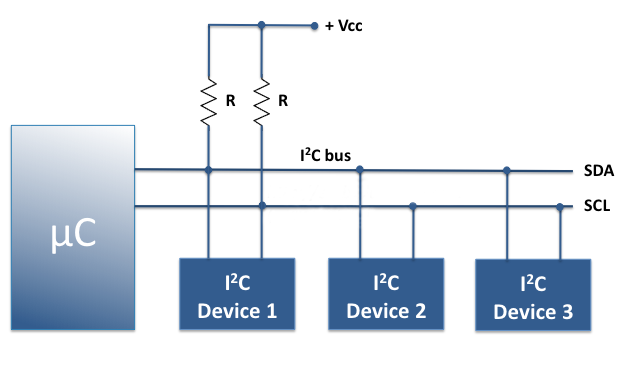
\includegraphics[width=6cm]{./figures/i2c-diagram.png}
 \caption{Sample \icc implementation (adapted from \emph{embedded-lab.com}).}
 \label{fig:i2c-implementation}
\end{figurehere}

Each \icc transaction is always initiated by the master which is in charge of
the bus for the entire duration of the transaction, meaning that it controls the
clock and generates the START and STOP sequences. The start and stop sequences
mark the beginning and the end of a transaction and are the only places where
the SDA line is allowed to change while the SCL is high.

All data are transfered one byte at a time. In 7-bit addressing mode, the slave
address occupies the seven most significant bits of the first byte, with the
least significant bit serving as a read/write flag to indicate whether data
will be written to the slave ('0') or data will be read from the slave ('1').
For every byte received, the slave device sends back an acknowledge bit.
Figure \ref{fig:i2c-implementation} shows an example of a typical \icc
transaction.

The \icc protocol supports multiple masters. In a multi-master environment two
or more masters may simultaneously attempt to initiate a data transfer.
In such a scenario, each master must be able to detect a collision and to follow
the arbitration logic that leeds to the election of a winner master. The winner
master can then safely begin its transaction.
The Nomadik NHK8815 platform, like most system designs, operates in a 
single-master environment.

\begin{figurehere}
 \centering
 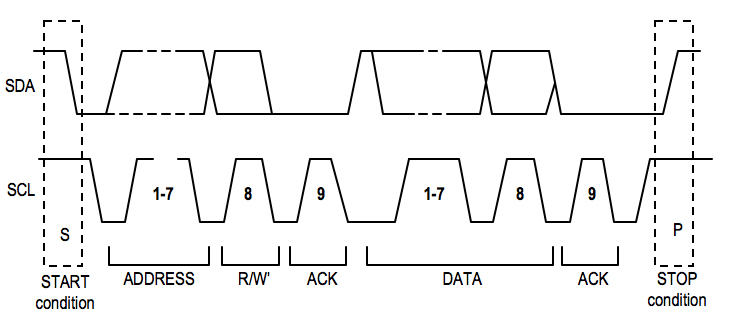
\includegraphics[width=8cm]{./figures/i2c-transaction.jpg}
 \caption{Sample \icc transaction (adapted from \emph{www.ermicro/blog}).}
 \label{fig:i2c-transaction}
\end{figurehere}

\emph{The Linux \icc subsystem}\\[6pt]
The Linux kernel \icc framework consists of a core layer where resides all the
routines and data structures available to bus drivers and client drivers
(figure \ref{fig:linux-i2c-subsystem}).
The core also provides a level of indirection that allows the underlying drivers
to change from one system to another without affecting \icc subsystem that
relies on them.

This philosophy of a core layer and its attendant benefits is an example of how
Linux helps portability. For instance, enabling \icc on a new platform (which is
precisely the objective of this project) requires only to design the
hardware-dependent components, namely the bus driver and the client drivers,
whereas the core layer needs not to be changed.

\begin{figurehere}
 \centering
 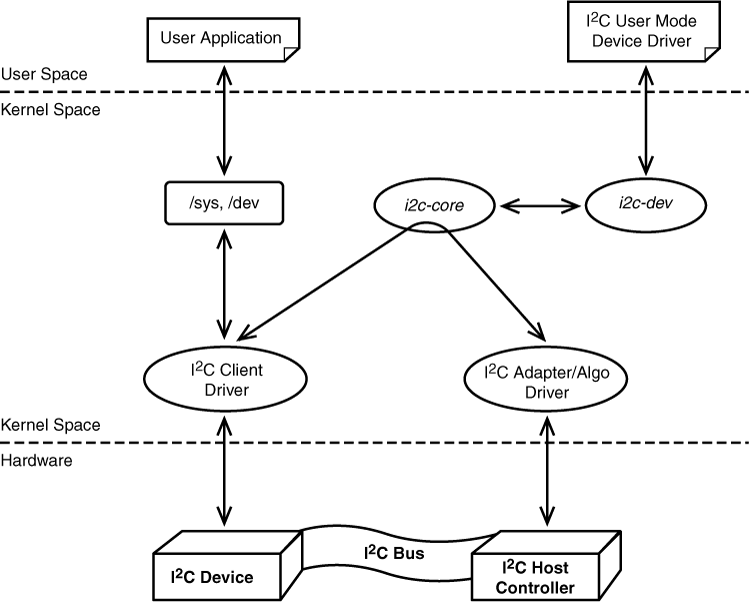
\includegraphics[width=7.5cm]{./figures/linux-i2c-subsystem.png}
 \caption{The Linux \icc subsystem (reprinted from \cite{venkateswaran2008eldd},
 		p. 236).}
 \label{fig:linux-i2c-subsystem}
\end{figurehere}



%-------------------------------------------------------------------------------
\subsection{The Nomadik NHK8815 platform}
\label{sec:nomadik_nhk8815_platform}
The NHK8815 is a full-featured evaluation board for the ST Microelectronics
Nomadik STn8815 (figure \ref{fig:nomadik-nhk8815}). It is a fan-less embedded
computer equipped with a wide range of peripheral devices including USB, UART,
LAN, WLAN, Bluetooth, FM radio, SIM card reader, SD/MMC card reader, color LCD
with touch screen controller, key-pad, video encoder, audio codec, FM radio,
three-axis accelerometer, etc..

\begin{figurehere}
 \centering
 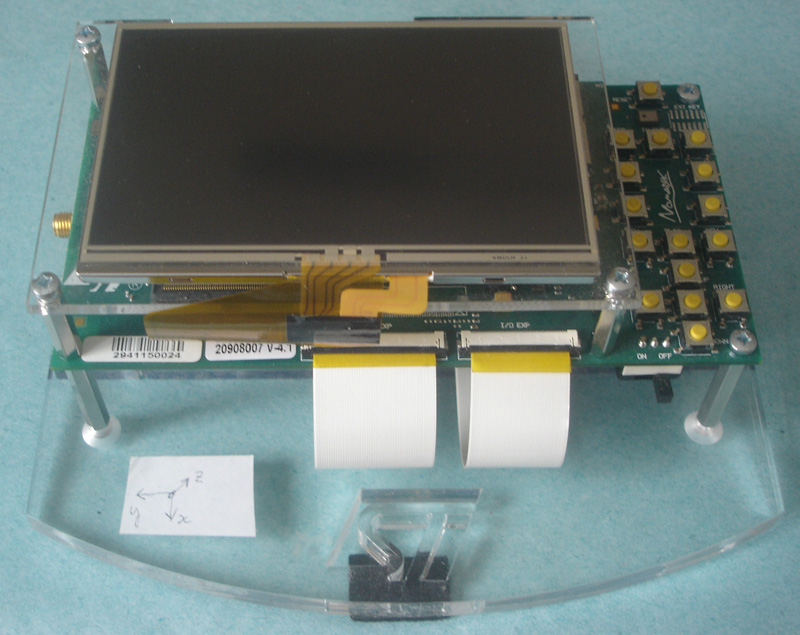
\includegraphics[width=8cm]{./figures/nomadik-nhk8815.jpg}
 \caption{The Nomadik NHK8815 evaluation board.}
 \label{fig:nomadik-nhk8815}
\end{figurehere}

The core of the board is the Nomadik STn8815 multimedia application processor.
The STn8815 is a \emph{System On Chip} that combines an ARM9 core up to 332MHz
with level-two cache to audio, video, imaging and graphics accelerators.

Among other interfaces, the STn8815 integrates two \icc high speed controllers
that support the physical and data-link layer of the \icc protocol.
Below is a list of the \icc controllers' main features:
\begin{packeditems}
	\item Slave transmitter/receiver and master transmitter/receiver modes.
	\item Standard (100kHz), fast (400kHz) and high-speed (3,4MHz) baud rates.
	\item 7-bit or 10-bit addressing.
	\item Compliance with \icc standards.
\end{packeditems}

In a traditional \icc bus topology such as the one in figure
\ref{fig:i2c-implementation}, the STn8815 \icc embedded controller plays the
role of the master. In order for the controller to access the \icc bus, a
corresponding driver must be implemented and registered with the \icc
subsystem. This step is covered in section \ref{sec:i2c_bus_driver},
"\nameref{sec:i2c_bus_driver}."

Because on the NHK8815 evaluation board the majority of the on-board peripheral
devices is connected to the STn8815 \icc bus 0, in this project I focus the
attention on this bus rather than on bus 1.
The table \ref{table:i2c-device-addresses} reports the list of devices on 
the \icc bus 0, with their 7-bit address.
Just like for the case of the bus driver, in order for each slave device
to function a corresponding driver must be registred to the \icc subsystem.
My choice for this project was the LIS3LV02DL, a MEMS inertial sensor mapped
at the address 1D on the Nomadik board.
The design of the LIS3LV02DL driver is detailed in section
\ref{sec:i2c_client_driver}, "\nameref{sec:i2c_client_driver}."\\[6pt]

\begin{tablehere}
	\centering
	\renewcommand{\arraystretch}{1.2}	
	\begin{tabular}{l l c}
		\hline
		Device type & Description & 7-bit address \\
		\hline
		STw5095 & Stereo audio codec & 1A \\
		LIS3LV02DL & Inertial sensor & 1D \\
		STw8009 & Video digital encoder	 & 21 \\
		TDA8023TT & Smart Card interface & 22,23 \\
		STw4811 & Power management & 2D \\
		STMPE2401 & Port expanders & 43,44 \\
		TSC2003IPW & Touch screen controller & 48 \\
		STw4102 & Battery charger & 70 \\
		\hline
	\end{tabular}
	\caption{NHK8815 \icc device address map.}
	\label{table:i2c-device-addresses}
\end{tablehere}



%-------------------------------------------------------------------------------
\subsection{Project setup}
\label{sec:project_setup}

The first step to the project is to get the Linux kernel source and to configure
it for the target board. Instead of  using a vendor supplied kernel such as like
STLinux, my personal strategy for this project was to work with the official
kernel from \emph{www.kernel.org}.
This decision was motivated by the need to keep the development process as neat
as possible, and to avoid performing tasks that are not strictly concerned with
the project.

It should be noted that the official kernel offers only limited support for the
Nomadik  NHK8815 platform.
This includes basic definitions and register addresses, interrupt management,
resource definitions and timers. The \icc interface can be used through the
generic drivers \emph{i2c-gpio} and \emph{i2c-algo-bit}, but no one of the
NHK8815 \icc slave devices is provided.

I cloned the git repository at kernel.org on a local machine folder
located \underline{outside} the project workspace. From the tag \emph{3.3}
I created a new branch called \emph{i2cdevel}, where to commit the kernel updates.
I generated one patch per commit. All patches are numbered in sequence and
stored in a folder \underline{inside} the project workspace called
\emph{linux-3.3.0-patches}.

One benefit of this approach is that the project workspace, which is a git
repository as required, also holds all the data needed to obtain the modified
kernel from the official one.
Table \ref{table:project-dir-layout} shows the project workspace layout.
In addition, to ease the project management I defined a set of environmental
variables. A list of them with their definition is presented in table
\ref{table:project-env-variables}.

Finally, a note about the root filesystem. It was built using BusyBox
version 1.18.4 (\cite{busybox}). More precisely, I used a tool called
\textbf{bbfs 1.3}, developed by \emph{Alessandro Rubini} and released under
GNU GPL license (see \cite{bbfs1.3} for details).\\

\begin{tablehere}
	\centering
	\renewcommand{\arraystretch}{1.2}	
	\begin{tabular}{l p{5.5cm}}
		\hline
		Variable & Decription \\
		\hline
		\texttt{PRJROOT} & The project root directory\\
		\texttt{KERNELDIR} & The root directory of the kernel source tree \\
		\texttt{PATCHESDIR} & The \emph{linux-3.3.0-patches} directory \\
		\texttt{ROOTFS} & The directory where is stored the target root
			filesystem \\
		\texttt{MODULESDIR} & The directory for temporary holding of the
			loadable driver modules \\
		\hline
	\end{tabular}
	\caption{Project environmental variables.}
	\label{table:project-env-variables}
\end{tablehere}


\begin{table*}
	\centering
	\renewcommand{\arraystretch}{1.2}	
	\begin{tabular}{p{5cm} p{11cm}}
		\hline
		Directory & Content \\
		\hline
		\texttt{linux-3.3.0-patches} & The patches to the Linux kernel and the 
			kernel configuration file \emph{.config}\\
		\texttt{drivers} & The bus driver and slave driver (one subfolder per
			each driver) \\
		\texttt{report} & The \LaTeX sources of this paper \\
		\texttt{script} & Shell scripts (copied to the root directory of the
			target filesystem) \\
		\texttt{tools} & User-space programs to evaluate the drivers (copied to
			the root directory of the target filesystem) \\
		\texttt{images} & The binary image of the kernel and the root
			filesystem \\
		\hline
	\end{tabular}
	\caption{Project directory layout.}
	\label{table:project-dir-layout}
\end{table*}




%%%%%%%%%%%%%%%%%%%%%%%%%%%%%%%%%%%%%%%%%%%%%%%%%%%%%%%%%%%%%%%%%%%%%%%%%%%%%%%%
\section{I2C client driver}
\label{sec:i2c_client_driver}

This section describes the design of the driver for the LIS3LV02DL inertial
sensor which equips the NHK8815 evaluation board.
The LIS3LV02DL is a three axes linear accelerometer that provides the measurement acceleration signals to the external world through an \icc interface.
The LIS3LV02DL driver was written before the bus driver. Its debug was possible
by using the gpio-based \icc bus driver available in the original kernel. Once
completed and tested, the LIS3LV02DL driver was then used for debugging the new
STN8815 \icc bus driver.\\



%-------------------------------------------------------------------------------
\subsection{Initialization and probing}
\label{sec:lis3_init_probe}

During initialization the driver registers itself with the \icc core. This
is achieved by populating a \keyword{struct i2c\_driver} and passing it
as argument to the function \keyword{i2c\_add\_driver()} as shown below.

\begin{lstlisting}[
	xleftmargin=15pt,
	frame = l,
	numbers=left,
	caption = {Registration of the LIS3LV02DL driver
		(from \emph{lis3lv02d-nhk8815.c}).},
	label = {list:lis3-i2cdrv-registration}
]
/* Device and driver names */
#define	DEVICE_NAME		"lis3lv02d"

/* I2C client structure */
static struct i2c_device_id lis3lv02d_idtable[] = {
  { DEVICE_NAME, 0 },
  {}
};
MODULE_DEVICE_TABLE(i2c, lis3lv02d_idtable);

static struct i2c_driver lis3lv02d_driver = {
  .driver   = {
    .name = DRIVER_NAME
  },
  .probe    = lis3lv02d_probe,
  .remove   = __devexit_p(lis3lv02d_remove),
  .id_table = lis3lv02d_idtable,
};

/* Module init */
static int __init lis3lv02d_init(void)
{
  return i2c_add_driver(&lis3lv02d_driver);
}
\end{lstlisting}

The structure \keyword{i2c\_driver} holds pointers to the probe function
and to the remove function that are executed respectively on device probing
and when the device is removed (if ever).
The \keyword{id\_table} member of the structure \keyword{i2c\_driver} informs
the \icc framework about which slave devices are supported by the driver.
In this case the only chip supported is named \keyword{lis3lv02d}.
The names of the supported devices are important for \emph{binding}, as
explained next.

The binding process consists of associating a device with a driver that can
control it. In embedded systems where the number of the \icc bus and the
devices connected to it are known for a fact, it is possible to declare in
advance the \icc slaves which live on the bus. This is typically done in the
board setup file, as shown below.

\begin{lstlisting}[
	xleftmargin=15pt,
	frame = l,
	numbers = left,
	caption = {Registration of the I2C devices (from \emph{board-nhk8815.c}).},
	label = {list:lis3-i2cdev-declaration}
]
/* I2C devices */
static struct i2c_board_info nhk8815_i2c_devices[] = {
  {
    I2C_BOARD_INFO("lis3lv02d", 0x1D),
    .irq = NOMADIK_GPIO_TO_IRQ(82),
    /* No platform data: use driver defaults */
  },
};

static void __init nhk8815_platform_init(void)
{
  ...
  /* Register I2C devices on bus #0 (scl0, sda0) */
  i2c_register_board_info(0, nhk8815_i2c_devices,
    ARRAY_SIZE(nhk8815_i2c_devices));
  ...
}
\end{lstlisting}

The \keyword{nhk8815\_platform\_init} function is executed on board startup
and, among other tasks, registers the \icc slave devices by invoking the
\keyword{i2c\_register\_board\_info} function with arguments that specify
the number of the bus (zero in this case) and the devices connected with it.
This is done through an array of \keyword{struct i2c\_board\_info}, each item
of which specifies the device name and the device address, with the former that
must match with the name registered by the driver in order for binding to succeed.
In this case \keyword{struct i2c\_board\_info} holds only one item which
corresponds to the LIS3LV02DL inertial sensor. Seeing that this sensor's chip
has an interrupt line tied to the cpu (gpio 82), the \keyword{irq} member is
also specified with the respective IRQ number. By means of another member
called \keyword{platform\_data} it is possible to define custom data for the
driver; if not specified like in this case, the driver uses its default
settings, as explained in section \ref{sec:lis3_settings}.

During boot the kernel looks for any \icc driver that has registered a matching
device name, that is "lis3lv02d". Upon finding such a driver, the kernel
ivokes its \keyword{probe()} function passing a pointer to the LIS3LV02DL
device as a parameter. This process is called \emph{probing}.

The probe function is responsible for the per-device initialization, that is
initializing hardware, allocating resources, and registering the device with
any appropriate subsystems. More in detail, the LIS3LV02DL probe function
takes the following actions:
\begin{packedenum}
	\item Allocate memory for a \keyword{struct lis3lv02d\_priv} private data
		structure.
	\item Load the device settings.
	\item Idendify the LIS3LV02DL chip.
	\item Configure the device hardware.
	\item Create the per-device sysfs nodes.
	\item If the free-fall feature is enadled, request the interrupt and
		register the IRQ for the free-fall detection.
	\item If the device polling feature is enabled, register the device with
		the input subsystem.
\end{packedenum}
On successful completion of all the above steps, meaning a successful probing,
the device is bound to the driver.


%-------------------------------------------------------------------------------
\subsection{Sysfs interface}
\label{sec:lis3_sysfs}

Sysfs is an in-memory virtual filesystem that provides a view of the kernel's
structured device model. It offers a convenient yet simple way to implement
functionality as sysfs attribute in the appropriate directory. An attribute
provides a way to map kernel data to files in sysfs: a single attribute maps to
a single file which can be readable, writable or both, depending on which
functionality it exports.

A driver wishing to use sysfs needs to register the sysfs attributes and implement
their respective functions. The table \ref{table:lis3-sysfs-attributes} shows
the list of sysfs nodes handled by the LIS3LV02DL driver. They are located in
\keyword{/sys/devices/platform/lis3lv02d/}.

\begin{tablehere}
	\centering
	\renewcommand{\arraystretch}{1.2}	
	\begin{tabular}{l c p{4cm}}
		\hline
		Attribute & Access & Function \\
		\hline
		\texttt{position} & r & Show the acceleration along the x,y,z axis \\
		\hline
		\texttt{enable} & r & Show the enable status of the device \\
						& w & Enable/disable the device \\
		\hline
		\texttt{ff\_enable} & r & Show the enable status of the free-fall 
					 			  feature \\
		\hline
		\texttt{poll\_enable} & r & Show the enable status of the polling
									feature \\
							  & w & Enable/disable the device polling \\
		\hline
		\texttt{read} & r & Read the register at the current address \\
					  & w & Set the current address for reading \\
		\hline
		\texttt{write} & w & Write a register. The low byte holds the register
							 value and the high byte holds the register address \\
		\hline
	\end{tabular}
	\caption{LIS3LV02DL sysfs attributes.}
	\label{table:lis3-sysfs-attributes}
\end{tablehere}

The figure \ref{fig:lis3-sysfs} shows a
dump of a shell session executed on the target board, providing a short
demonstration of how to play with the LIS3LV02DL sysfs interface.

The \keyword{cat enable} command returned 'n', meaning that the device was
disabled.
Turning the device on is achieved by the command \keyword{echo 1 > enable}.
The \keyword{cat position} command returned the values 56, -4, 1043 which
correspond to to acceleration along the x-axis, y-axis and z-axis measured
in $mg$. \keyword{cat ff\_anable} showed that the free-fall feature is enabled.
Finally, the last two commands perform a reading at the address 0F; the answer
is 3A.
\footnote{0F is the address of the \keyword{WHO\_AM\_I} register which holds
the device identification number (3A for the LIS3LV02DL chip)}.

\begin{figurehere}
 \centering
 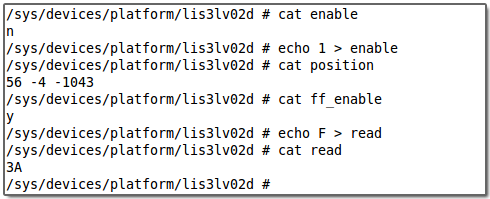
\includegraphics[width=7.5cm]{./figures/dump-lis3lv02d-sysfs.png}
 \caption{Example of usage of the LIS3LV02DL sysfs interface.}
 \label{fig:lis3-sysfs}
\end{figurehere}


%-------------------------------------------------------------------------------
\subsection{Device polling}
\label{sec:lis3_poll}

Generally speaking \emph{polling} is a technique in which one device periodically
monitors multiple other devices or makes requests from those devices (e.g. check
their state). In this project's context, the polling device is the target
cpu while the LIS3LV02DL inertial sensor is the device being polled.

To implement the polling feature the LIS3LV02DL driver registers itself with the
kernel's \emph{input subsystem}; this involves registering \keyword{open()},
\keyword{close()} and \keyword{poll()} call-back functions, specifying
the polling interval, setting up the type of events involved, etc.
The input subsystem takes care of calling the \keyword{poll()} function at the
specified rate, registering any event notification reported by the driver and
dispatching it to the user-space via sysfs in
\keyword{/dev/input/eventX} ('X' is a numeric identifier assigned when the
driver registers with the input core).
A demonstration of how the device polling works is given in the section
\ref{sec:evdev-testing}.

The listing \ref{list:lis3-poll-enable} shows the sequence of instructions
required to registers with the input core. The driver executes them upon
enabling polling. It allocates the input device, installs the callback
function pointers (lines 8-10), programs the ABS events related to the x,y,z
acceleration data (lines 14-17), and registers the input device (line 26).
Lines 20 through 23 relates to the free-fall feature which is explained in
the next section.

\begin{lstlisting}[
	xleftmargin=15pt,
	frame = l,
	numbers = left,
	caption = {Device registration with the input subsystem
		(from \keyword{lis3lv02d\_poll\_enable()} in
		\emph{lis3lv02d-nhk8815.c}).},
	label = {list:lis3-poll-enable}
]
struct input_polled_dev *input_polled;
struct input_dev *input;

/* Allocate memory for the input device */
input_polled = input_allocate_polled_device();

/* Setup input parameters */
input_polled->open = lis3lv02d_open;
input_polled->close = lis3lv02d_close;
input_polled->poll = lis3lv02d_poll;
input = input_polled->input;

/* Setup ABS input events */
set_bit(EV_ABS, input->evbit);
set_bit(ABS_X, input->absbit);
set_bit(ABS_Y, input->absbit);
set_bit(ABS_Z, input->absbit);

/* Setup KEY event for free-fall (only if enabled) */
if (priv->ff_enabled) {
  set_bit(EV_KEY, input->evbit);
  set_bit(KEY_FREE_FALL, input->keybit);
}

/* Register input polled device */
input_register_polled_device(input_polled);
\end{lstlisting}

To disable polling the driver unregisters the input device and frees its
previously allocated memory (listing \ref{list:lis3-poll-disable}).

\begin{lstlisting}[
	xleftmargin=15pt,
	frame = l,
	numbers = left,
	caption = {Device unregistration
		(from \keyword{lis3lv02d\_poll\_disable()} in 
		\emph{lis3lv02d-nhk8815.c}).},
	label = {list:lis3-poll-disable}
]
/* Unregister input device */
input_unregister_polled_device(priv->input_polled);
input_free_polled_device(priv->input_polled);
\end{lstlisting}

Upon loading the LIS3LV02DL driver, the polling function may be either enabled
or not enabled, depending on whether the default or custom settings were used
(see section \ref{sec:lis3_settings} for details).
Once the driver is up and running, the polling can be enabled/disabled via the
sysfs \keyword{poll\_enable} file, as detailed in the previous section.


%-------------------------------------------------------------------------------
\subsection{Free-fall detection}
\label{sec:lis3_free-fall}
The LIS3LV02DL may be configured to generate an inertial wake-up/free-fall
interrupt signal when a programmable acceleration threshold is crossed at least
in one of the three axes.

The LIS3LV02DL driver installs a threaded ISR to handle the free-fall detection.
Upon receiving an interrupt request the driver reads the acceleration values
from the sensor and notifies an appropriate event to the input core for being
dispatched to the user-space.
Indeed the driver relies on the input subsystem to "inform" the user-space
about a free-fall event. This implies that the device polling be enabled.

Usage of the free-fall feature can be enabled only statically (i.e at compile
time) either by adjusting the driver's defaults or by passing custom settings
from the board initialization code (through \keyword{platfom\_data}).
From user-space the free-fall enable status can be seen via the sysfs
\keyword{ff\_enable} file (see table \ref{table:lis3-sysfs-attributes}).

If the free-fall is enabled, the driver's \keyword{probe()} registers the IRQ
number (as provided by the device) and installs its respective threaded ISR
(lines 10-15 of listing \ref{list:lis3-irq-register}).

\begin{lstlisting}[
	xleftmargin=15pt,
	frame = l,
	numbers = left,
	caption = {Registration of the free-fall IRQ
		(from \keyword{probe()} in \emph{lis3lv02d-nhk8815.c}).},
	label = {list:lis3-irq-register}
]
/* Get IRQ (only if free-fall is enabled) */
if (pdata->free_fall_cfg & LIS3_FF_ALL) {
  ...
  /* Register IRQ */
  err = request_threaded_irq(client->irq, NULL,
    lis3lv02d_isr_thread,
    IRQF_TRIGGER_RISING | IRQF_ONESHOT,
    DEVICE_NAME, priv);
  ...
  priv->ff_enabled = true;
}
\end{lstlisting}

The free-fall is notified in form of a KEY event. As for all the input
events this requires two steps: registering with the input subsystem
and reporting upon detection of free-fall.
The former being executed by \keyword{lis3lv02d\_poll\_enable()} (lines 20-23
of listing \ref{list:lis3-poll-enable}), and the latter being handled by the
free-fall ISR as shown below.

\begin{lstlisting}[
	xleftmargin=15pt,
	frame = l,
	numbers = left,
	caption = {Notification of a free-fall KEY event
		(from \keyword{lis3lv02d\_isr\_thread()} in \emph{lis3lv02d-nhk8815.c}).},
	label = {list:lis3-isr}
]
/* Report free-fall (KEY) event */
input_report_key(input, KEY_FREE_FALL, true);
input_report_key(input, KEY_FREE_FALL, false);
input_sync(input);
\end{lstlisting}


%-------------------------------------------------------------------------------
\subsection{LIS3LV02DL settings}
\label{sec:lis3_settings}

The customization of the LIS3LV02DL settings is done based on \emph{platform data}.
These are data attached to a platform device, that are completely specific to
a given device. It allows the board initialization file to transmit detailed and
custom information about the device to the driver.
In this project's context, the platform data is represented in form of a
\keyword{lis3lv02d\_nhk8815\_platform\_data} structure
(listing \ref{list:lis3-paltform-data}) which allows to set a number of LIS3LV02DL parameters including the acceleration full-range (2g or 6g), free-fall settings,
polling interval, etc..

\begin{lstlisting}[
	xleftmargin=15pt,
	frame = l,
	numbers = left,
	caption = {LIS3LV02DL driver's platform data
		(from \emph{lis3lv02d-nhk8815.h}).},
	label = {list:lis3-paltform-data}
]
/* Platform data */
struct lis3lv02d_nhk8815_platform_data {
  unsigned char device_cfg;
  unsigned char free_fall_cfg;
  unsigned int free_fall_threshold;
  unsigned char free_fall_duration;
  unsigned int poll_interval;
}
\end{lstlisting}

The board initialization code may omit to transmit custom data, as it relies on
the driver using its default settings. This is precisely the solution adopted for
this project as shown in listing \ref{list:lis3-i2cdev-declaration}.
One may choose the other way round and set up the \keyword{platform\_data}
member of \keyword{i2c\_board\_info} to point to a 
\keyword{lis3lv02d\_nhk8815\_platform\_data} structure with custom settings.

Upon probing the driver checks whether \keyword{platform\_data} holds a valid
pointer and, if this is the case, loads the custom settings. Otherwise it uses
the default values. The code responsible for this action is reported in listing
\ref{list:lis3-check-platform-data}.

\begin{lstlisting}[
	xleftmargin=15pt,
	frame = l,
	numbers = left,
	caption = {Loading of LIS3LV02DL platform  data
		(\keyword{lis3lv02d\_probe()} in \emph{lis3lv02d-nhk8815.c}).},
	label = {list:lis3-check-platform-data}
]
/* Save pointer to platform data */
pdata = client->dev.platform_data;
if (!pdata) {
  dev_info(&client->dev,
  "no platform data, using defaults\n");
  pdata = &lis3lv02d_default_init;
}
\end{lstlisting}

In listing \ref{list:lis3-platform-data-defaults} are shown the default settings
for the LIS3LV02DL device as they are defined in \emph{lis3lv02d-nhk8815.c}.

The driver was built as a module and manually loaded into the kernel using the
\keyword{insmod} program. Upon successful load the driver delivers an information
message about its settings to the kernel as shown in figure \ref{fig:lis3-insmod}.
The last command, \keyword{lsmod}, produces the list of modules currently loaded
into the kernel (only \keyword{lis3lv02d-nhk8815} in this example).

\begin{lstlisting}[
	xleftmargin=15pt,
	frame = l,
	numbers = left,
	caption = {LIS3LV02DL default setup
		(from \emph{lis3lv02d-nhk8815.c}).},
	label = {list:lis3-platform-data-defaults}
]
/* LIS3LV02DL default configuration */
static const struct lis3lv02d_nhk8815_platform_data
	lis3lv02d_default_init = {

  .device_cfg = LIS3_ODR_40HZ | LIS3_FS_2G,
  .poll_interval = 500,
  .free_fall_cfg = LIS3_FF_XL | LIS3_FF_YL | LIS3_FF_ZL,
  .free_fall_threshold = 600,
  .free_fall_duration = 5,	/* 1/ODR [s] */
};
\end{lstlisting}

\begin{figure*}
% \centering
 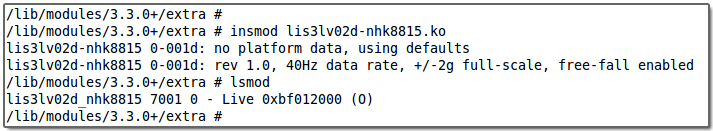
\includegraphics[width=11.8cm]{./figures/dump-lis3lv02d-insmod.png}
 \caption{Message showed upon loading LIS3LV02DL module with default settings.}
 \label{fig:lis3-insmod}
\end{figure*}



%%%%%%%%%%%%%%%%%%%%%%%%%%%%%%%%%%%%%%%%%%%%%%%%%%%%%%%%%%%%%%%%%%%%%%%%%%%%%%%%
\section{I2C bus driver}
\label{sec:i2c_bus_driver}

As mentioned in section \ref{sec:nomadik_nhk8815_platform} the STn8815 processor
integrates two \icc controllers that can be programmed to work in standard, fast
or high-speed mode. It is designed to operate in a multi-master environment,
either as a master or as a slave. However, because the STn8815 is the only master
on board, and seeing that at this time Linux only operates \icc in master mode, 
the \icc bus driver presented here supports master mode only.


%-------------------------------------------------------------------------------
\subsection{Initialization and probing}
\label{sec:adapter_init_probe}
Initializing and probing the STn8815 \icc bus driver is performed in a similar
way as for LIS3LV02DL client driver (section \ref{sec:lis3_init_probe}), with
the major difference being that the former uses a \emph{platform bus}.

The platform bus requires that any \icc \emph{adapter} (or equivalently
\emph{controller})
\footnote{The two terms are interchangeable in meaning and refer to the
peripheral device that drives the bus (i.e. the master device)}.
which is controlled by the bus driver be registered using a \keyword{platform\_device} structure.
This structure represents the bus adapter and provides information such as the
device name, the device resources and the adapter number, to the bus driver.

Usually the registration of the \icc adapters with the platform bus is
performed by the board initialization file, as the information needed are
highly board specific. And this case is no exception.

The listing \ref{list:i2c-reg-platform-dev} shows the part relevant to this
matter, taken from \emph{arch/arm/mach-nomadik/i2c-8815nhk.c}. Because of the
STn8815 has two \icc adapters, two platform devices need to be defined: one for
bus 0 and one for bus 1.
In this example the former uses the platform data mechanism to customize the
driver settings, while to the latter relies on the driver's defaults
(see section \ref{sec:adapter_settings} for details about the driver settings).

The \keyword{resource} and \keyword{num\_resources} fields allow to define
the device resources (for brevity not shown here). These include the
definition of the memory area (base address and size) and the interrupt number.

\begin{lstlisting}[
	xleftmargin=15pt,
	frame = l,
	numbers = left,
	caption = {Registration of the \icc adapter with the platform bus
		(from \emph{i2c-8815nhk.c}).},
	label = {list:i2c-reg-platform-dev}
]
/* first bus: i2c0 */
static struct platform_device nhk8815_i2c_dev0 = {
  .name		= "stn8815_i2c",
  .id		= 0,
  .resource	= &nhk8815_i2c_resources[0],
  .num_resources = 2,
  .dev		= {
    .platform_data = &nhk8815_i2c_dev0_data,
  },
};

/* second bus: i2c1 */
static struct platform_device nhk8815_i2c_dev1 = {
  .name		= "stn8815_i2c",
  .id		= 1,
  .resource	= &nhk8815_i2c_resources[2],
  .num_resources	= 2,
  /* No platform data: use driver defaults */
};

static int __init nhk8815_i2c_init(void)
{
  ...
  platform_device_register(&nhk8815_i2c_dev0);
  ...
  platform_device_register(&nhk8815_i2c_dev1);
  ...
}
arch_initcall(nhk8815_i2c_init);
\end{lstlisting}

On the driver's side, the registration with the platform bus is achieved by
populating a \keyword{struct  platform\_driver} and passing it to the
macro \keyword{module\_platform\_driver()} as argument (listing
\ref{list:i2c-reg-platform-drv}).
The platform bus simply compares the \keyword{driver.name} member against
the name of each device, as defined in the \keyword{platform\_device} data
structure (listing \ref{list:i2c-reg-platform-dev}); if they are the same
the device matches the driver.

\begin{lstlisting}[
	xleftmargin=15pt,
	frame = l,
	numbers = left,
	caption = {Registration of the \icc bus driver with the platform bus
		(from \emph{i2c-stn8815.c}).},
	label = {list:i2c-reg-platform-drv}
]
#define DRIVER_NAME 	"stn8815_i2c"

static const struct dev_pm_ops stn8815_i2c_pm_ops = {
  SET_RUNTIME_PM_OPS(stn8815_i2c_runtime_suspend,
                     stn8815_i2c_runtime_resume,
                     NULL)
};

static struct platform_driver stn8815_i2c_driver = {
  .probe  = stn8815_i2c_probe,
  .remove = __devexit_p(stn8815_i2c_remove),
  .driver = {
    .name  = DRIVER_NAME,
    .owner = THIS_MODULE,
    .pm	= &stn8815_i2c_pm_ops,
  },
};
module_platform_driver(stn8815_i2c_driver);
\end{lstlisting}

As usual, binding a device to a driver involves calling the driver's 
\keyword{probe()} function passing a pointer to the device as a parameter.
The sequence of operations performed on probing are the following:
\begin{packedenum}
	\item Get the device resource definitions
	\item Allocate the appropriate memory and remap it to a virtual address
		for being accessed by the kernel
	\item Load the device settings.
	\item Configure the device hardware.
	\item Register with the power management system.
	\item Create the per-device sysfs nodes.
	\item Request the interrupt and	register the IRQ.
	\item Set up the \keyword{struct i2c\_adapter} and register the adapter
		with the \icc core.
\end{packedenum}

Once all the above steps successfully complete the driver is bounded to the
devices representing the two STn8815 \icc controllers.


%-------------------------------------------------------------------------------
\subsection{Data transfer}
\label{sec:adapter_data_transfer}

In the Linux \icc subsystem a bus driver consists of an \emph{adapter driver}
and an \emph{algorithm driver}. The motivation behind this further division is
to improve the software reuse and to allow portability. In fact, an algorithm
driver is intended to contain general code that can be used for a whole class
of \icc adapters, while each specific adapter driver either depends on one
algorithm driver, or includes its own implementation.

However, while having a generic algorithm that works for multiple adapters is
suitable for many cases, in embedded systems, where each \icc bus
adapter has its own way of interfacing with the processor and the bus,
it is usual to develop the adapter driver together with its corresponding
algorithm driver. This is also the case of the STn8815 \icc bus driver.

The bus driver registers with the \icc subsystem by using a
\keyword{struct i2c\_adapter} that is instantiated and initialized by the
driver's \keyword{probe()} function, as shown in listing
\ref{list:i2c-adapter-reg}.
The \keyword{i2c\_adapter} structure's \keyword{algo} member is set up to
point to a \keyword{struct i2c\_algorithm} which in turn holds two pointers:
\begin{packeditems}
	\item \keyword{master\_xfer} points to the function that implements the
		actual \icc transmit and receive algorithm.
	\item \keyword{functionality} points to a function that returns the
		features supported by the \icc adapter.
\end{packeditems}

\begin{lstlisting}[
	xleftmargin=15pt,
	frame = l,
	numbers = left,
	caption = {Registration of the \icc adapter (from \emph{i2c-stn8815.c}).},
	label = {list:i2c-adapter-reg}
]
/* I2C algorithm structure */
static struct i2c_algorithm stn8815_i2c_algo = {
  .master_xfer   = stn8815_i2c_xfer,
  .functionality = stn8815_i2c_func,
};

/* Probe function */
static int __devinit stn8815_i2c_probe
	(struct platform_device *pdev)
{
  ...
  adap = kzalloc(sizeof(struct i2c_adapter),
         GFP_KERNEL);
  ...
  adap->algo = &stn8815_i2c_algo;
  ...
  err = i2c_add_numbered_adapter(adap);
  ...
}
\end{lstlisting}

To communicate with a client the \icc subsystem offers two class of functions:
one for \icc plain communication which includes \keyword{i2c\_master\_send()},
\keyword{i2c\_master\_recv()} and \keyword{i2c\_transfer()}, and a second one
that uses SMBus commands
\footnote{SMBus is a subset of \icc}.
However, whichever method is used, the data transfer relies on the bus driver's
function pointed to by \keyword{master\_xfer}, as the \icc core ultimately calls
this function for the actual transfer to take place.

As shown in listing \ref{list:i2c-adapter-reg}, \keyword{stn8815\_i2c\_xfer()}
is the transfer function installed by the STn8815 \icc bus driver.
This function receives an array of messages as argument and process
them in sequence by calling \keyword{stn8815\_i2c\_xfer\_rd()} or
\keyword{stn8815\_i2c\_xfer\_wr()} depending respectively on whether the message
being processed is marked for read or write.
Once all message have been sent \keyword{stn8815\_i2c\_xfer()} succesfully
returns, otherwise, upon detecting a communication error, aborts the transmission
and returns an appropriate error code.

The STn8815 \icc bus driver uses the STn8815 \icc controller's interrupt
capability to handle the data transfer. More precisely it uses interrupts to
trigger the completion of a transaction and to detect a bus error. Handling
these interrupts is in charge of \keyword{stn8815\_i2c\_isr()} interrupt service
routine (ISR).
Its role is to identify the interrupt source, complete the transaction
by reporting the result to the \emph{task-level}
\footnote{\emph{Task-level} refers to code not running in interrupt context
(as opposed to \emph{interrupt-level})}
function that initiated it (either \keyword{stn8815\_i2c\_xfer\_wr()} or
\keyword{stn8815\_i2c\_xfer\_rd()}), and to clear the interrupt condition from
the \icc controller.

A \emph{completion variable} is used to synchronize between the task-level
function and the ISR. The former initiates the transmission and waits on the
completion variable while the \icc controller performs the transaction; upon
completion, the controller issues an interrupt request which is processed by
\keyword{stn8815\_i2c\_isr()}; once it has accomplished its job, upon returning
from interrupt, \keyword{stn8815\_i2c\_isr()} uses the completion variable to
wake up the task-level function.
Additionally, a timeout is specified to limit the time spent by the task-level
function on waiting on the completion variable.
The whole process is depicted in the sequence diagram of figure
\ref{fig:i2c-trans-seq-diag}.

The listing \ref{list:i2c-completion-sync} shows how the synchronization
mechanism is implemented.
The completion variable is dynamically created and initialized via
\keyword{init\_completion()} (line 7). Afterwards, a call to
\keyword{wait\_for\_completion\_timeout()} (line 11) suspends the task until
either the ISR signals the completion by calling \keyword{complete()} (line 28)
or the timeout expires.  In either case the return value is tested for error
conditions.

\begin{lstlisting}[
	xleftmargin=15pt,
	frame = l,
	numbers = left,
	caption = {Task-level and ISR synchronization using a completion variable
		(from \emph{i2c-stn8815.c}).},
	label = {list:i2c-completion-sync}
]
/* I2C master read */
static int stn8815_i2c_xfer_rd(
    struct i2c_adapter *adap,
    struct i2c_msg *pmsg, bool stop)
{
  ...
  /* Initialize completion */
  init_completion(&dev->msg_complete);
  ...

  /* Wait for completion */
  i = wait_for_completion_timeout(&dev->msg_complete,
                                  I2C_TIMEOUT);
  if (i < 0)
    return i;
  if (i == 0) {
    dev_err(dev->dev, "Controller timeout\n");
    return -ETIMEDOUT;
  }
  ...
}

/* ISR */
static irqreturn_t stn8815_i2c_isr(int irq,
	void *dev_id)
{
  ...
  /* Complete */
  complete(&dev->msg_complete);
  return IRQ_HANDLED;
}

\end{lstlisting}

\begin{figure*}
 \centering
 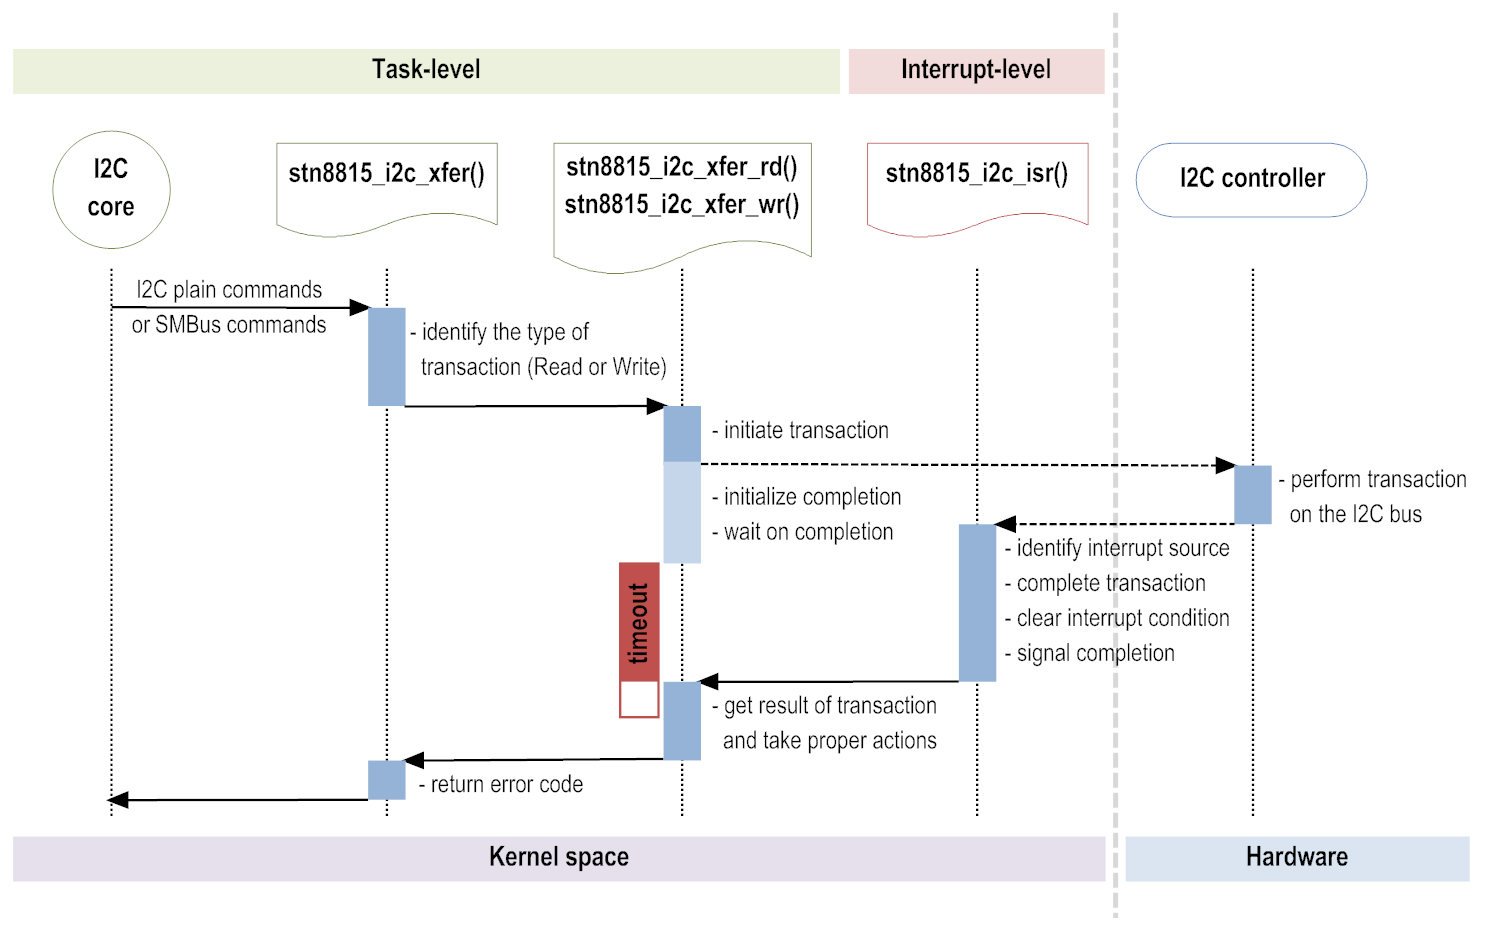
\includegraphics[width=16cm]
 	{./figures/i2c-data-transfer-seq-diag.png}
 \caption{Sequence diagram of an \icc transaction.}
 \label{fig:i2c-trans-seq-diag}
\end{figure*}


%-------------------------------------------------------------------------------
\subsection{Power management}
\label{sec:adapter_power_management}

The \icc bus driver relies on the power management infrastructure of the Linux
kernel to achieve run-time power savings. To use this feature the kernel needs
to be configured with "Runtime power management" (\keyword{CONFIG\_PM\_RUNTIME})
option enabled.

The functions that implements the driver's power saving policy are registered
upon registering the driver with the platform bus (refer to listing
\ref{list:i2c-reg-platform-drv} on page \pageref{list:i2c-reg-platform-drv}).
This is done by initializing the \keyword{driver.pm} member of the
\keyword{platform\_driver} structure with a pointer to
\keyword{struct dev\_pm\_ops} which in turn holds the address of the driver's
power management functions.

When the power management subsystem in Linux determines that the \icc adapter
is to be suspended (resumed) it calls \keyword{stn8815\_i2c\_runtime\_suspend()}.
This function simply disables the \icc controller.  
When the adapter is to be resumed, \keyword{stn8815\_i2c\_runtime\_resume()} is called and consequently the \icc controller is re-enabled.

The power management framework creates for the \icc adapter 0 a set of sysfs
nodes that allow to query or modify its power status. They are all located in \keyword{/sys/devices/platform/stn8815\_i2c.0/power/}.

For example, typing \keyword{cat runtime\_status} returns the adapter's power
status, while the command \keyword{echo 'off' > control} disables the adapter's
runtime power management.


%-------------------------------------------------------------------------------
\subsection{\icc bus adapter settings}
\label{sec:adapter_settings}

As for LIS3LV02DL, the \icc bus driver receives custom settings from the board
initialization code via the platform data mechanism.
Looking back at listing \ref{list:i2c-reg-platform-dev}, the adapter 0 uses a
custom setup (line 8), while the adapter 1 relies on the driver's defaults
(line 18).

The platform data of the \icc adapter is defined in \emph{i2c-stn8815.h} and
reported in listing \ref{list:i2c-adapter-platform-data}.
It is represented in form of a \keyword{i2c\_stn8815\_platform\_data} structure
and allows to specify the speed mode (standard, fast or high-speed), 
the bus filtering and the master code.

\begin{lstlisting}[
	xleftmargin=15pt,
	frame = l,
	numbers = left,
	caption = {STN8815 \icc bus driver's platform data
		(from \emph{i2c-stn8815.h}).},
	label = {list:i2c-adapter-platform-data}
]
/* Platform data */
struct i2c_stn8815_platform_data {
  unsigned char filter;
  unsigned char speed;
  unsigned int  master_code;
}
\end{lstlisting}

The driver loads the platform data on probing and, if not provided, it uses the default setup as defined by \emph{nhk8815\_i2c\_default\_init}
(listing \ref{list:i2c-adapter-data-defaults}).
The figure \ref{fig:i2c-adapter-insmod} shows the information message sent to
the kernel by the driver on successful load.

\begin{lstlisting}[
	xleftmargin=15pt,
	frame = l,
	numbers = left,
	caption = {STN8815 \icc bus adapter default setup
		(from \emph{i2c-stn8815.c}).},
	label = {list:i2c-adapter-data-defaults}
]
/* STN8815-I2C platform data default */
static struct i2c_stn8815_platform_data
	nhk8815_i2c_default_init = {
  .filter	= I2C_STN8815_FILTER_NONE,
  .speed	= I2C_STN8815_SPEED_STANDARD,
  .master_code = 0,
};
\end{lstlisting}

\begin{figure*}
% \centering
 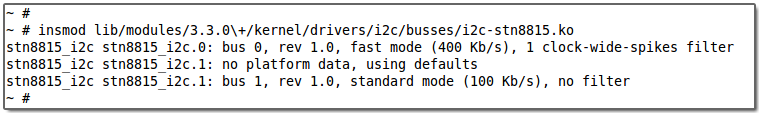
\includegraphics[width=12.4cm, height=1.7cm]{./figures/dump-adapter-insmod.png}
 \caption{Message showed upon loading the STN8815 \icc bus driver module with
 	default settings.}
 \label{fig:i2c-adapter-insmod}
\end{figure*}


%%%%%%%%%%%%%%%%%%%%%%%%%%%%%%%%%%%%%%%%%%%%%%%%%%%%%%%%%%%%%%%%%%%%%%%%%%%%%%%%
\section{Testing}
\label{sec:testing}
% x contesto dei test (remote console)
% x lis3 via /sys (partially already explained in previous sections)
% x lis3 via /dev (evtest)
% - i2c-dev (don't forget citations) using 'i2cexe' tool and i2cprobe script

As I said in section \ref{sec:project_setup} my choice for this project was
to work with the official kernel, which yet lacks many drivers necessary to
fully operate the Nomadik NHK8815 board. Clearly this choice influenced the
way the design process was conducted.
For example, the on-board LCD display and keypad were not used for interfacing
to the system because of the absence of the respective drivers in the kernel.
Instead, I connected to the target board through a serial line (UART) and
interfaced with it using a terminal emulator. This was achieved by configuring
appropriately the bootloader installed on the target, namely U-Boot
(\cite{uboot}).

A number of tools and scripts were used to help testing the drivers throughout
the design process. They all run in user-space and interface with the Linux
kernel, each one using either the \emph{sysfs} interface, the \emph{evdev}
interface or the \emph{i2c-dev} interface.
The figure \ref{fig:whole-driver-system} shows a view of the whole driver
system including the tools mentioned above.
This section describes some simple techniques that allows to test the drivers
using these tools. The tests are classified based on the type of interface 
they rely on.

\begin{figure*}
 \centering
 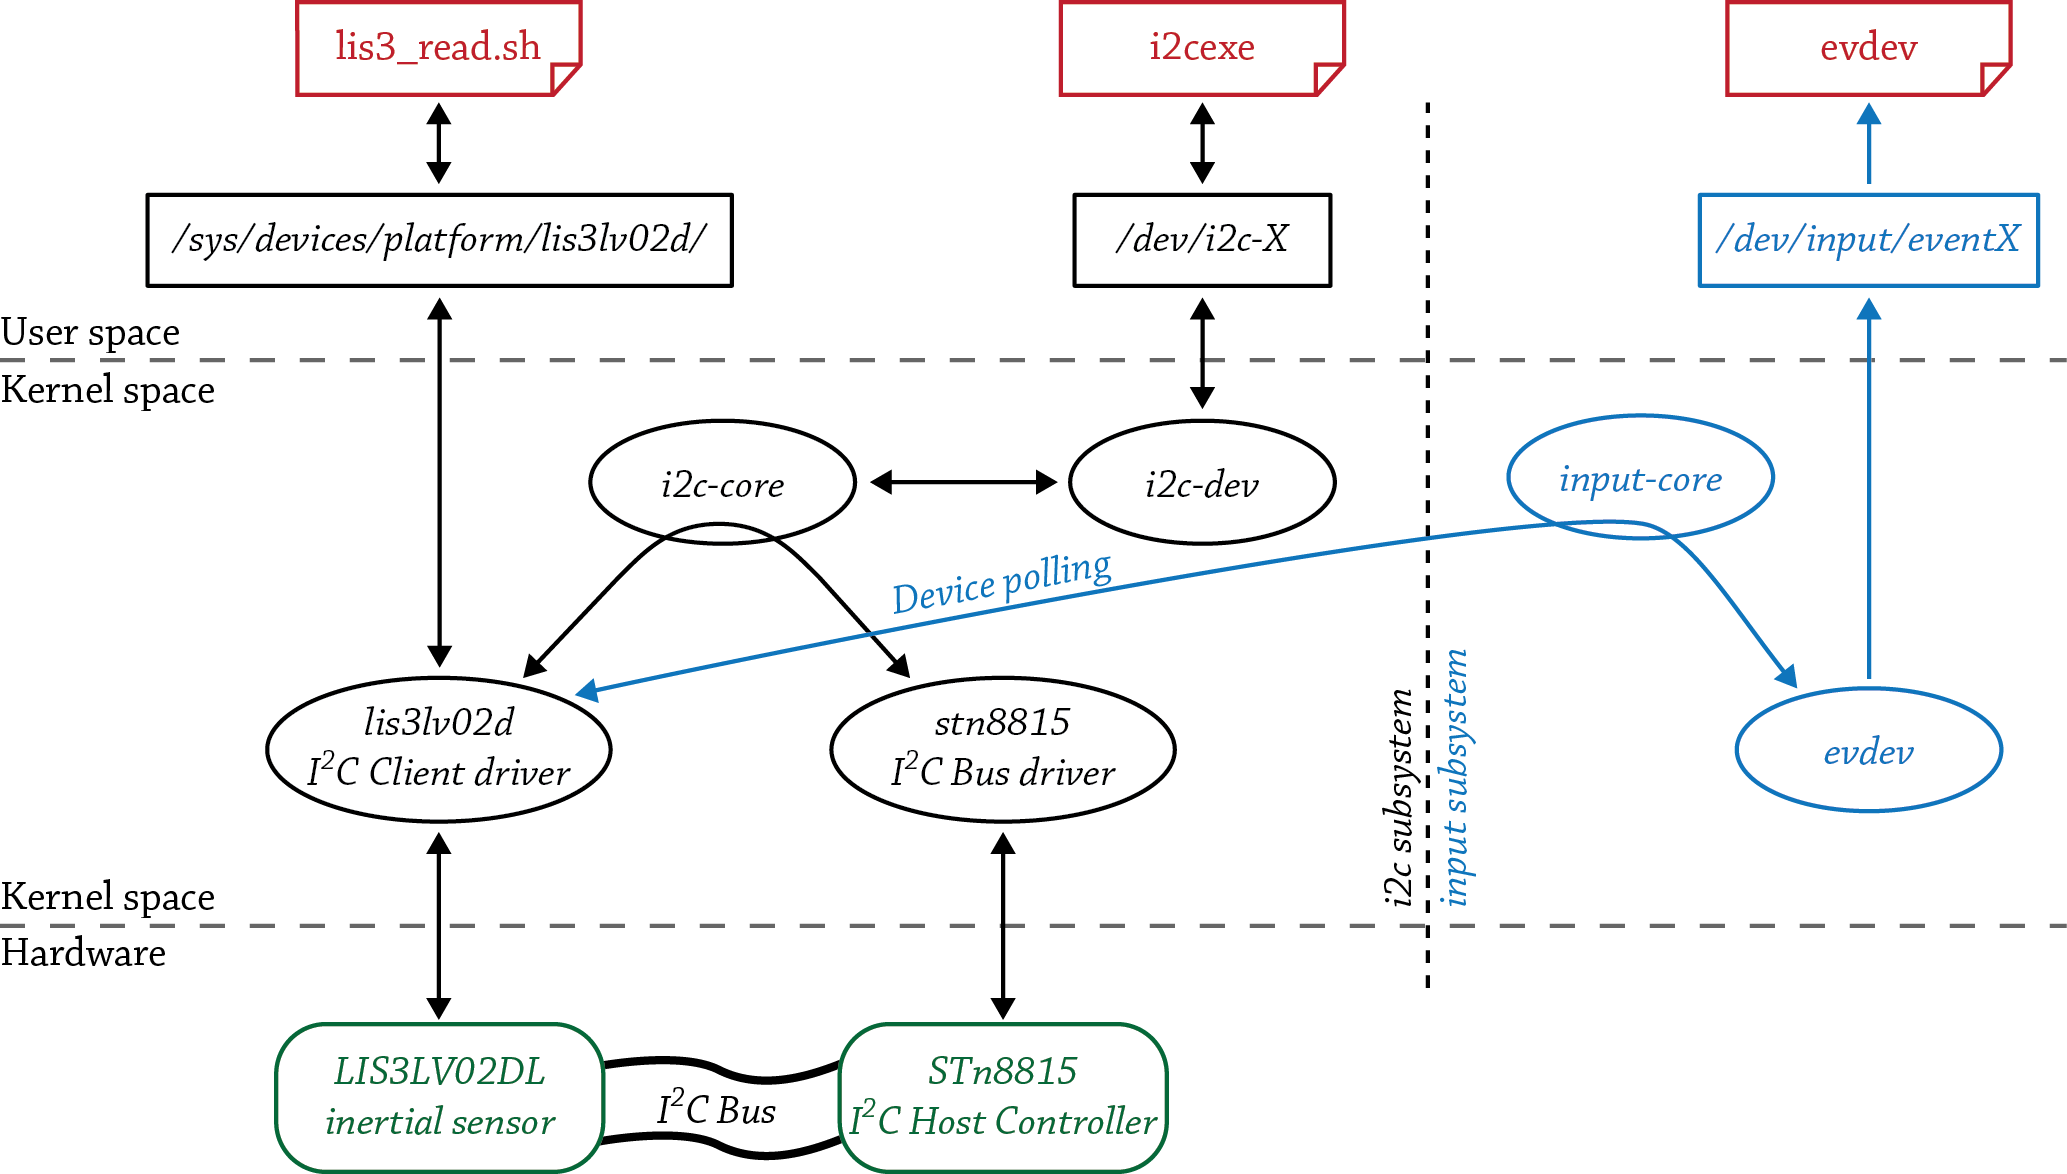
\includegraphics[width=15cm]{./figures/nhk8815-whole-driver-system.png}
 \caption{The LIS3LV02DL inertial sensor and STn8815 \icc host controller
 	complete driver structure.}
 \label{fig:whole-driver-system}
\end{figure*}


%-------------------------------------------------------------------------------
\subsection{Testing via the \emph{sysfs} interface}
\label{sec:sysfs-testing}
The usage the LIS3LV02DL sysfs interface was previously described in section
\ref{sec:lis3_sysfs}.
This interface turns out to be useful also for debugging activity even
during the early stages of design, when most of the driver functions are yet
to be implemented.
An example of this is represented by the sysfs nodes \keyword{read} and
\keyword{write} which were designed solely to assist debugging (in fact they
are available only if it is defined the constant \keyword{LIS3LV02D\_DEBUG}
in the driver source file). 

\keyword{read} and \keyword{write} together are used in the shell script
\emph{lis3\_read.sh} to implement a simple technique for testing the drivers.
This script allows to read a user defined set of registers of the accelerometer.
It has the following syntax:
\begin{verbatim}
	lis3_read.sh <filename>
\end{verbatim}
where \keyword <filename> refers to a file holding the list of registers with
their respective address. Below is an example of this file (from \emph{lis3\_registers} provided along with the script):

\begin{lstlisting}[language=bash]
# ------------------------------------
# Register name   Register Address
#                   (hex format)
# ------------------------------------
CTRL_REG1               20
CTRL_REG2               21
CTRL_REG3               22
STATUS_REG              27
FF_WU_CFG               30
FF_WU_SRC               31
FF_WU_THS_L             34
FF_WU_THS_H             35
FF_WU_DURATION          36
\end{lstlisting}

For each register in the list \emph{lis3\_read.sh} performs two steps:

\begin{packedenum}
	\item Sets up the address of the register via sysfs \keyword{write}.
	\item Reads the address content via sysfs \keyword{read}.
\end{packedenum}

Below is the output of the script when invoked with \emph{lis3\_registers}
as a command line parameter.

\begin{figurehere}
 \centering
 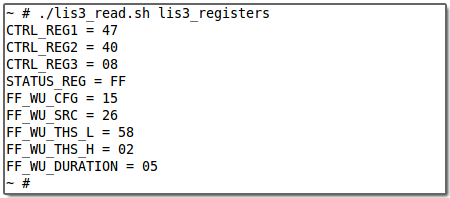
\includegraphics[width=7cm]{./figures/dump-lis3-read.png}
 \caption{Output of the script \emph{lis3\_read.sh} with \emph{lis3\_registers}
 	as a register file.}
 \label{fig:lis3-read}
\end{figurehere}


%-------------------------------------------------------------------------------
\subsection{Testing via the \emph{evdev} interface}
\label{sec:evdev-testing}

In Linux the directory \emph{/dev} is conventionally used to store the
device files, i.e. files representing interfaces for device drivers. They
allow user programs to access hardware devices through their respective
drivers. Linux classifies drivers in three categories: character, block and
network drivers.

LIS3LV02D driver fits in neither of the above three categories, as it doesn't
create a corresponding device file.
Consequently it's not possible for a user program to directly operate on the
accelerometer via a node in \emph{/dev}.
Instead, upon enabling the device polling, an indirect access is provided by
the \emph{evdev} interface of the input subsystem via a
\keyword{/dev/input/eventX} node.
The accelerometer driver reports the events to the input core, which in turn
writes them to this file in an appropriate format for being processed by a user
program.

An example of such a program is \emph{evtest} \cite{evtest}. It is a free
software released under GNU GPL license and available online in many versions;
1.23 is the one used in this project. This tool allows to display the events
reported by an input device. Below it is shown a sample output from evtest on
the target system.

\begin{figurehere}
 \centering
 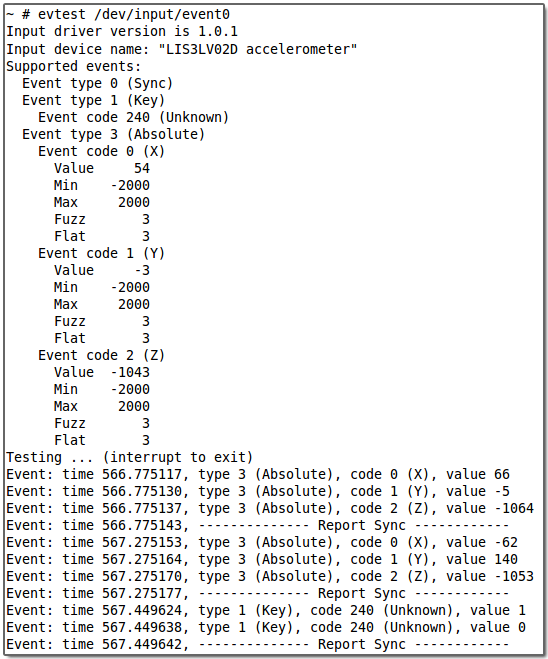
\includegraphics[width=8cm]{./figures/dump-evtest.png}
 \caption{Example of usage of \emph{evtest}.}
 \label{fig:evtest-dump}
\end{figurehere}

Initially evtest shows some information about the input device and its supported
event types (Sync, Key and Absolute) then, starting from the line
\keyword{Testing ... (interrupt to exit)}, keeps displaying any data from the
event node.
Since the accelerometer driver terminates each notification by a "sync" event, 
from the sample dump we can identify three distinct groups of events.
Both the first and the second groups represent absolute events corresponding to
the acceleration measured along the three cartesian axes.
The third group regards the free-fall which is reported as a key press
(value 1) and release (value 0) sequence of events.



%-------------------------------------------------------------------------------
\subsection{Testing via the \emph{i2c-dev} interface}
\label{sec:i2c-dev-testing}

The \emph{i2c-dev} interface was designed to allow driving the \icc devices from
user space. Each \icc adapter is assigned a number, say \keyword{X}, and a
corresponding device file is created in \keyword{/dev/i2c-X}.
It is indeed possible for a user mode driver to access an \icc client by
operating the adapter \keyword{X} through its node \keyword{/dev/i2c-X}.

However, in this project the \emph{i2c-dev} interface was used with the only
purpose of testing the \icc bus driver. To this aim I designed a user program
called \emph{i2cexe} which allows to transmit \icc messages to a generic client.
In the above scenario this tool plays the role of a user mode device driver
without effectively being a real driver, as it performs only a single \icc 
transaction (either read or write).

It should be noticed that, as opposed to the previous methods, this test
requires no \icc client driver whatsoever, i.e. the test applies to the \icc bus driver only.
Additionally, the Linux kernel must be configured with with "I2C device interface" (\keyword{CONFIG\_I2C\_DEV}) option enabled.




%%%%%%%%%%%%%%%%%%%%%%%%%%%%%%%%%%%%%%%%%%%%%%%%%%%%%%%%%%%%%%%%%%%%%%%%%%%%%%%%
\section{Conclusion}

TODO.



%%%%%%%%%%%%%%%%%%%%%%%%%%%%%%%%%%%%%%%%%%%%%%%%%%%%%%%%%%%%%%%%%%%%%%%%%%%%%%%%
% Add all references without citing
\nocite{nxp-i2c-spec}
\nocite{linux-kernel-archive}


% We suggest the use of JabRef for editing your bibliography file (Report.bib)
\bibliographystyle{splncs}
\bibliography{Report}

\end{multicols}
\end{document}
